\documentclass[a4paper]{amsbook}
\usepackage[utf8]{inputenc}
\usepackage{parskip}
%\usepackage{amsmath}
%\usepackage{amssymb}
%\usepackage{amsthm}
\usepackage{pgf}
\usepackage{tkz-graph}
\usepackage{tikz}
\usetikzlibrary{arrows,automata,cd,positioning,shapes}

\newtheorem{definition}{Definition}[section]
\newtheorem{lemma}{Lemma}[section]
\newtheorem{corollary}{Corollary}[section]
\newtheorem{theorem}{Theorem}[section]
\newtheorem{maintheorem}{Main Theorem}[section]

\newcommand{\dderives}[1]{\underset{#1}{\Rightarrow}}
\newcommand{\derives}[1]{\underset{#1}{\overset{*}{\Rightarrow}}}
\newcommand{\pathcat}[1]{\mbox{$\mathcal{W}(#1)$}}
\newcommand{\fa}[1]{\mbox{$\mathcal{#1}$}}
\newcommand{\faequiv}[1]{\underset{\fa{#1}}{\equiv}}
\newcommand{\lang}[1]{\mbox{$L_{\mathcal{#1}}$}}
\newcommand{\edge}[1]{\stackrel{#1}{\longrightarrow}}
\newcommand{\pocymon}[1]{\mbox{${#1}^{(*)}$}}
\newcommand{\transrem}[1]{(Translator's remark: #1)}

\title{Formal Languages\\An automata-theoretic introduction}
\author{Prof.\ Dr.\ Günter Hotz\\Universität des Saarlandes
\and Dr.\ Klaus Estenfeld\\Universität des Saarlandes
\and English translation by\\Dipl.-Inform.\ Armin Reichert\\Alumnus Universität
des Saarlandes}
\makeindex
\begin{document}
\maketitle
\chapter*{Preface}

This book is in essence the second edition of the book Hotz/Walter,
''Automatentheorie und Formale Sprachen 2, Endliche Automaten''. As it has been
completely reworked, it really is a new edition.

While in the first edition only the theory of finite automata has been treated,
in this edition also an introduction into the theory of context-free languages
is given. This was only possible in the available space frame because
of an automata-theoretic treatment of the theory.

Such a foundation of the theory has already been proposed by Goldstine in 1977
and has been sketched in various of his lectures. The motivation for developing
my lecture, from which this book originates, in this way however is not based on
 his proposal. It has almost automatically been arosen from the
work of the French school. I want to emphasize here the book by Jean Berstel on
transductions. Mr.\ Berstel finally pointed my to the work of Goldstine.

I fully support Goldstine's opinion that it would be worth rethinking the
whole theory of formal languages along this automata-theoretic lines.

This book is only an introduction into the theory of formal languages. The
interested reader who wants to gets a deeper understanding of the theory or who
wants to get a different look into it is pointed to the books by Ginsburg,
Harrison or Salomaa. Relations to applications can be found in books on complier
design.

Dr.\ Klaus Estenfeld worked out my lecture ''Formal Languages 1'' which I held 
on this topic in 1980/81 to become the foundation of this book and he made a
number of additions at some places.

Dipl.-Math.\ Bernd Becker carefully read the manuscript and contributed with his
proposals to the success of this book.

The publisher as well as the editors of the series earn our thanks for their
patience of waiting for the second edition.

Saarbrücken, August 1981

\vspace{2em}
{\em Günter Hotz}

\tableofcontents
\chapter*{Introduction}

There are several reasons for the interest in the theory of formal languages in
computer science. Practical problems as they arise in the context of the
specification and translation of programming languages find an exact
description in the theory of formal languages and so get accessible to an exact
treatment. Generation processes definable by formal languages can be interpreted as 
non-deterministic automata which is as a generalized notion of a computer.

These kinds of generalizations in general are easier to understand than
deterministic algorithms which contain more details that do not reflect the
original problem but the necessity to unambiguosly define the algorithm. This is
part of the reason of the difficulty to prove the correctness of programs in
an understandable way. On the other side, the proof of correctness for grammars
or other mechanisms for generating languages offers the possibility to study correctness proofs
on simpler objects.

The theory of formal languages in this respect contains the theory of
algorithms but most often only the theory of {\bf context-free} languages is
treated because of her extraordinary simplicity and beauty.

In the light of the theory stand different methods for defining
formal language classes, studying their word and equivalence problems and
putting them into different hierarchical classifications.

The generation processes themselves become objects of interest in the theory
because the generation process of a language in case of programming languages
is related to the semantics of the programs.

Of course, in the context of such a pocket book we have to make a strong
selection of topics concerning language classes, generation processes as well as
basic questions. In doing so, we let us guide by the intention to keep the
formal machinery rather small.

Because the theory of finite automata is the foundation for the whole theory of
formal languages, we start our book with this topic. In developing this theory
we do not consider the technical realization of finite automata by logical
circuits and binary storage devices but rather focus on the basic algorithm however it is realized.
 
Our intuitive notion of finite automaton consists of a finite, oriented graph whose 
edges are labeled with the symbols from the input alphabet of the automaton. 
Depending on the input word we look for a path in the graph labelled with that
word. If the end point of such a path, originating from the dedicated ''start point'' 
of the automaton, is a member of the set of ''end points'', our automaton
''accepts'' the word and doesn't do otherwise.

We prove the equivalence of this concept with the other known methods of
defining finite automata. We prove the usual closure properties of languages
defined by finite automata. Additionally we investigate the relation between
deterministic and non-deterministic automata and also 2-way automata.

It is possible to generalize this theory in the direction of considering not
only the free monoid of strings (words) over a finite alphabet but also
arbitrary monoids.

By considering finite automata with output, which means to attach a second label
at the graph edges, we get the theory of {\bf rational transducers}. An
extensive treatment of the theory of general transductions can be found in the book by
Berstel.

Here we restrict ourselves to some special generalizations of the free monoid
(of words), namely the {\bf free group}, the {\bf H-group} (where the relation
$x x^{-1} = 1$ holds for $x$ from the generating system, but not $x^{-1} x = 1$) and the
{\bf polycyclic monoid} (in addition to $x x^{-1} = 1$ it holds $x y^{-1} = 0$
for $x \neq y$ and $0 x = x 0 = 0$ for $x,y$ from the generating system).

By investigating the transductions from free monoids into the polycyclic
monoids one gets a smooth transition from the theory of finite automata into the
theory of context-free languages.

The corresponding construction of the theory of context-free languages leads to
a simple path to the most important representation theorems. This includes the
theorems of Chomsky-Schützenberger, Shamir and Greibach. Also for the
transformation into Greibach normal form we get a simple and efficient
algorithm.

In the same easy way as for finite automata one can prove the known closure
properties for context-free languages.

In the end we also prove the equivalence of this representation with the usual
representation of context-free languages using context-free grammars.

Our development of the theory is very close to the one repeatedly recommended by
Goldstine since 1977, but its origins are independent from him. The difference
is that we prove Greibach's representation theorem by making our automaton deterministic,
namely by switching from output monoids to {\bf monoid rings}. Doing that you
get the theorem of Shamir in a natural way and from this the theorem of Greibach.

From the theorem of Shamir you can get quite easily the algorithm of Valiant for
deciding the word problem of context-free languages. Because of lack of space
this could not be included into this book, the same holds for the treatment of
the  deterministic languages.

We want to emphasize another advantage of this development of the theory: As
known, the exact formalization of the notion of ''derivation'' when using
grammars brings some difficulties. In our theory, the ''derivation tree''
corresponds to a path in our graph.

Maybe the use of non-free monoids is initially a problem for readers not used to
it. But it seems to be the case that defining context-free
languages in that way supports the intuition. For example, the usage of ''syntax
diagrams'' for the definition of programming languages gives some evidence for
this.

Because we judge the former as rather important, we want to explain it on a
specific example, namely the so-called {\bf Dyck language}.

The {\bf Dyck language} $D(X_k)$ contains the correctly nested bracket sequences
over $k$ different pairs of brackets, where $k \in \mathbb{N}$.

A formal definition of $D(X_k)$ is as follows:

Let $X_k = \{ x_1, \ldots, x_k \}$ be an alphabet of $k$ elements. Define
$\bar{X}_k = \{ \bar{x}_1, \ldots, \bar{x}_k \}$ such that $\bar{x}_i$ is regarded as the
closing bracket for $x_i$.

Then it holds:

\begin{enumerate}
  \item $\epsilon \in D(X_k)$
  \item $u, v \in D(X_k) \Rightarrow u \cdot v \in D(X_k)$
  \item $u \in D(X_k) \Rightarrow x_i \cdot u \cdot \bar{x}_i \in D(X_k),\quad
  \forall i = 1, \ldots, k$
  \item $D(X_k)$ is minimal with (1), (2) and (3). 
\end{enumerate}

For $D(X_k)$ we get the following syntax diagram:
%TODO: Fix diagram

\begin{center}
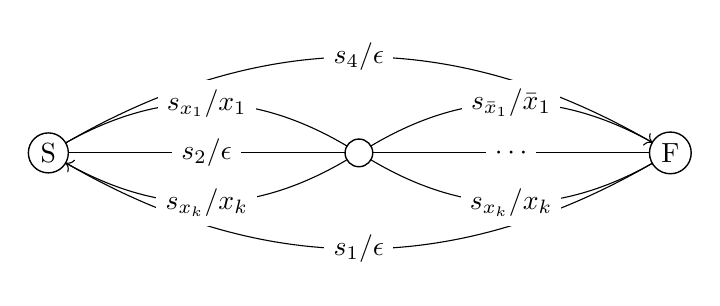
\begin{tikzpicture}[node distance = 10em]
\tikzset{VertexStyle/.append style = {minimum size = 1em}}
\tikzset{EdgeStyle/.append style = {->, bend left}}
\tikzset{LabelStyle/.style = {fill=white}}
\node[VertexStyle](S){S};
\node[VertexStyle,right=of S](V){ }; 
\node[VertexStyle,right=of V](F){F};
\draw[EdgeStyle](S) to node[LabelStyle]{$s_4/\epsilon$} (F);
\draw[EdgeStyle](F) to node[LabelStyle]{$s_1/\epsilon$} (S);
\path[]
	(S)	edge[bend left] 	node[LabelStyle] {$s_{x_1}/x_1$} (V)
	(S)	edge 							node[LabelStyle] {$\cdots$} (V)
	(S)	edge[bend right] 	node[LabelStyle] {$s_{x_k}/x_k$} (V)
	(V)	edge[bend left] 	node[LabelStyle] {$s_{\bar{x}_1}/\bar{x}_1$} (F)
	(V)	edge 							node[LabelStyle] {$\cdots$} (F)
	(V)	edge[bend right] 	node[LabelStyle] {$s_{x_k}/x_k$} (F)
	(V) edge							node[LabelStyle] {$s_2/\epsilon$} (S)
	;
\end{tikzpicture}
\end{center}

If we consider all labellings of paths from $S$ to $F$ we get of course also
words not contained in $D(X_k)$, for example $x_1 x_2 \bar{x}_k$ or $x_1
\bar{x}_1 \bar{x}_2$ etc.

We have to guarantee that we get Dyck words only. To do that, we define a
homomorphism from the path category of the graph into the polycyclic monoid over
$X_k \cup \bar{X}_k$ such that the homomorphic images of the paths from $S$ to
$F$ have a special form, for example they have to be equal to the unit of the
polycyclic monoid.

Let us consider the word
\[ x_1 x_2 \bar{x}_2 \bar{x}_1 x_2 \bar{x}_2 \in D(X_2), \]
then we have different paths
\[s_{x_1} s_2 s_{x_2} s_{\bar{x}_2} s_3 s_{\bar{x}_1} s_1
s_{x_2} s_{\bar{x}_2} \] 
and 
\[s_{x_1} s_2 s_{x_2} s_{\bar{x}_2} s_3
s_{\bar{x}_1} s_3 s_2 s_{x_2} s_{\bar{x}_2}\]
which both have this word as their label and we can easily define a
homomorphism in the sense above.

We get different paths in our graph leading to the acceptance of the same word.

The problem to construct a graph such that for each word in the accepted
language exactly one path exists leads to the existence of the {\bf
deterministic} finite automaton with storage.

\transrem{This type of automaton is also known as ''monoid-automaton''
and seems to get more attention nowadays. Some results from this book have also
been redetected, see for example \cite{doi:10.1080/00927870802243580},
\cite{Render}.}

\chapter{Mathematical Foundations}
\section{Notations, basic notions}

In this first section we want to define the elementary notions that are used
throughout the whole book. We use the usual notions
\[ \mathbb{N} = \{ 0, 1, 2, \ldots \}\ \mbox{for the natural numbers} \]
\[ \mathbb{Z} = \{ \ldots, -2, -1, 0, 1, 2, \ldots \}\ \mbox{for the integer
numbers} \]
\[ \mathbb{Q} = \{ \frac{a}{b} \mid a,b \in \mathbb{Z}, b \neq 0 \}\ \mbox{for
the rational numbers } \]

For the set operations we use $\cup$ for the union and $\cap$ for the
intersection. Also $A \subset B$, $a \in A$, $a \not\in A$, $\bar{A}$, $A - B$,
$A \times B$ and $\emptyset$ have their usual meaning. For the power set of a
set $A$ we write $2^A$ or $Pot(A)$. $Card(A)$ denotes the cardinality of $A$.
Logical implication is denoted by $\Rightarrow$.

{\bf Mappings} are denoted as $f : A \rightarrow B$, in that case $f$ is a
total mapping. We write $Q(f) = A, Z(f) = B$. Here $Q$ stands for ''Quelle'' (source)
and $Z$ for ''Ziel'' (target).

If $f: A \rightarrow B, g : B \rightarrow C$ are mappings, then $f \circ g : A
\rightarrow C$ is the composed mapping that one gets by applying $f$ first and
then $g$, i.e. $(f \circ g)(a) = g(f(a))$. If $f:A \rightarrow B$ and $C
\subset A$, then $f(C) = \{ f(c) \mid c \in C \}$.

A subset $R \subset A \times B$ is called a {\bf relation} between $A$ and $B$.
$R_f \subset A \times B$ with $R_f = \{ (a,b) \mid f(a) = b \}$ is the relation
{\bf induced by} mapping f or the {\bf graph} of $f$.

Let $f : A \rightarrow B$ be a mapping, $A_1 \subset A$ and $g : A_1 \rightarrow
B$ a mapping. $f$ is called the {\bf continuation} of $g$ if $f(a_1) = g(a_1),
a_1 \in A_1$. In this case we also write $f \mid _{A_1} = g$ (in words: $f$
restricted to $A_1$).

A {\bf semi-group} consists of a set $M$ an an associative operation on that
set, usually denoted as a multiplication. If a semi-group is commutative, we
also use ''$+$'' instead of ''$\cdot$''.

A semi-group is a {\bf monoid} if $M$ contains a neutral element. We often
denote it with $1_M$ or shortly $1$. In the commutative case we often write $0$
instead of $1$.

For $A,B \subset M$ we denote by $A \cdot B = \{ a b \mid a \in A, b \in B \}$
the {\bf complex product} of $A$ and $B$.

$A \subset M$ is a {\bf submonoid} of $M$ if the follwoing holds: $1_M \in A$
and $A$ is closed under the operation of $M$.

For an $A$, the set $A^*$ defined as follows, is the smallest submonoid of $M$
which contains $A$. More specific,
\[
		A^* = \bigcap_{M' \in M(A)} M'	
\]
where $M(A) = \{ M' \subset M \mid M'$ is a submonoid of $M, A \subset M' \}$.

It is easy to see that
\[
		A^* = \bigcup_{n \geq 0} A^n\ \mbox{with}\ A^0 = \{1\}\ \mbox{and}\ A^{n+1} =
		A^n \cdot A
\]

In the same sense the notion $A^+ = A^* - \{1\}$ is defined for semi-groups. $A$
is called the {\bf generation system} of $A^*$ and $A^+$ resp.

A special meaning for us is assigned to the set of ''words'' (string) over a
fixed alphabet $A$. We understand as words the finite sequences of elements from
the alphabet $A$ as for example $(a,b,d,a,c)$ for alphabet $A = \{ a,b,c,d \}$.

We define
\[
WORD(A) := \{\epsilon\} \cup A \cup (A \times A) \cup (A \times A \times A) \cup
\ldots
\]
as the set of words (strings) over $A$. The symbol $\epsilon$ denotes the {\bf
empty word} over $A$, that is $A^0 = \{\epsilon\}$.

If $w, v \in WORD(A)$ then $w \cdot v$ is the word over $A$ which you get by
concatenating $w$ and $v$, more formally:
\[
\mbox{If}\ w = (a_1,\ldots,a_k), v = (a_{k+1},\ldots,a_n)\ \mbox{then}\ w \cdot
v = (a_1, \ldots, a_n)
\]

With this operation $WORD(A)$ becomes a monoid which is usually also denoted
with $A^*$. This is slightly inconsistent because for the first definition of
the $*$-operator it holds $(A^*)^* = A^*$ but for the second usage of the
$*$-operator it holds $(A*)^* \neq A^*$.

The following example should clarify that: Let $A = \{a,b,c\}$ and let $(a,b,a)$
and $(b,a) \in A^*$.
\[(a,b,a)\cdot(b,a) = (a,b,a,b,a) \in A^*,\ \mbox{but}\]
\[((a,b,a),(b,a)) \in (A^*)^*\ \mbox{but}\ \notin A^*\].


Instead of $(a)$ we write just $a$. In this sense it holds $A \subset A^*$. This
also holds in the sense of the first definition of $A^*$.

If $w = (w_1,\ldots,w_n)$ we denote with $|a| = n$ the {\bf length} of $w$.
Obviously it holds: $|w \cdot v| = |w| + |v|$ and $|\epsilon| = 0$.

The {\bf mirror word} $w^R$ of a word $w = (w_1,\ldots,w_n)$ is the word
$(w_n,\ldots,w_1)$. $\epsilon^R = \epsilon$. It holds: $(w \cdot v)^R =
v^R \cdot w^R$.

In $A^*$ the reduction rules hold, i.e.
\begin{enumerate}
  \item $w \cdot x = w \cdot y \Rightarrow x = y$
  \item $x \cdot w = y \cdot w \Rightarrow x = y$
\end{enumerate}

We define {\bf left} and {\bf right quotient}:
\[ B^{-1} \cdot A = \{ v\ |\ \exists u \in B, w \in A : u \cdot v = w \} \]
and $A \cdot B^{-1}$ in the same way.

Because of the reduction rules it holds:
\[ \{w\}^{-1} \cdot \{v\}\ \mbox{and}\ \{w\}^{-1} \cdot \{v\}\ \mbox{resp. are
either empty or contain a single element.} \]

If $\{w\}^{-1} \cdot \{v\}$ is not empty we call $w$ a {\bf prefix} of $v$. If
$\{w\} \cdot \{v\}^{-1} \not= \emptyset $, we call $v$ a {\bf suffix} of $w$. In
the future we will always write just $w$ instead of $\{w\}$ and also $w$ is
prefix of $v$ if $w^{-1} \cdot v \not= \emptyset$.


\section{Monoid homomorphisms and congruence relations}

\begin{definition}[monoid homomorphism]
A {\bf monoid homomorphism} (short: homomorphism) from a monoid $M$ to a monoid
$S$ is a mapping $\Phi : M \to S$ with the following properties:
\begin{enumerate}
  \item $\Phi(m_1 \cdot m_2) = \Phi(m_1) \cdot \Phi(m_2), \quad m_1, m_2 \in M$
  \item $\Phi(1_M) = 1_S$
\end{enumerate}
\end{definition}

It can be easily shown: if $M_1 \subset M$ is a submonoid of $M$, then
$\Phi(M_1)$ is a submonoid of $S$. If $S_1$ is a submonoid of $S$, then
$\Phi^{-1}(S_1)$ is a submonoid of $M$.

A monoid homomorphism $\Phi : M \to S$ is called
\begin{description}
  \item[monomorphism] if $\Phi$ is injective
  \item[epimorphism] if $\Phi$ is surjective
  \item[isomorphism] if $\Phi$ is bijective
\end{description}

Homomorphisms $\Phi : M \to M$ are called {\bf endomorphisms}, isomorphisms
$\Phi : M \to M$ are called {\bf automorphisms}.

Monoids $M$ and $S$ are called {\bf isomorphic}, if there exists an
isomorphism between $M$ and $S$.

Of course, a homomorphism cannot be defined arbitrarily on a monoid $M$.
Thus the following two questions arise:
\begin{enumerate}
  \item If $M_1 \subset M$ is a submonoid and $\Phi_1 : M_1 \to S$ is an arbitrary
mapping. When is it possible to extend $\Phi_1$ to a homomorphism $\Phi
: M \to S$\ ?
	\item If $\Phi_1, \Phi_2$ both are homomorphisms from $M$ to $S$ which
	coincide on $M_1 \subset M$. In which way can $\Phi_1$ and $\Phi_2$ be
	different? 
\end{enumerate}

The answer to this question of course depends on the structure of $M_1$. If
$M_1 = \{ 1_M \}$ then $\Phi$ is determined uniquely on $M_1$ but there is
little information on the relation between $\Phi_1$ and $\Phi2$.

The following two simple theorems which can be found in introductory algebra
books are holding:
\begin{enumerate}
  \item If $M_1$ is a generating system of $M$ and $\Phi_1, \Phi_2 : M \to S$
  both are monoid homomorphisms which coincide on $M_1$, then $\Phi1 = \Phi_2$.
  \item If $A$ is a set and $M = A^*$, and $\Phi_1 : A \to S$ is an arbitrary
  mapping, then there exists exactly one continuation $\Phi$ from $\Phi_1$ which
  is a monoid homomorphism from $A^*$ to $S$.
\end{enumerate}

\begin{definition}[free generating system, free monoid]
A subset $A \subset M$ is called a {\bf free generating system} of $M$, if each
mapping $\Phi_1 : A \to S$, where $S$ is an arbitrary monoid, can be continued
to a monoid homomorphims in a unique way. A monoid with a free generating system
is called a {\bf free monoid}.
\end{definition}

$A^*$ therefore is a free monoid and $A$ is a free generating system of $A^*$.

It holds also: If $A$ is a free generating system of $M$ and $A^*$ is the monoid
of words (string) over $A$, then $A^*$ and $M$ are isomorphic.

A free monoid has at most one free generating system. From that we can see that
the length $|w|$ of a word $w \in A^*$ can be defined in a unique way for any
free monoid.

The length mapping $L$ is an example for a monoid homomorphism $L : A^* \to
\mathbb{N}$.

If $\Phi : M \to S$ is a monoid homomorphism, then the sets 
\[\{ \Phi^{-1}(s) \mid s \in S \} \subset Pot(M)\]
form a monoid isomorphic to $\Phi(M)$.

We want to handle now the following question:

Let $M$ be a monoid, $L \subset M$ be any subset of $M$. Does there exist a
monoid $S$ and a homomorphism $\Phi : M \to S$ with the following property:
There exists an $s \in S$ with $L \subset \Phi^{-1}(s)$?

Of course, there always exists such an $S$: Choose $S = \{1\}$ and $\Phi(M) =
\{1\}$.

Therefore we strengthen our task: Find $S$ and $\Phi$ such that $L \subset
\Phi^{-1}(S)$ and for each other homomorphism $\Psi$ with that property holds:
$L \subset \Psi^{-1}(S') \Rightarrow \Phi^{-1}(S) \subset \Psi^{-1}(S')$.

We want to describe $L$ as close as possible by a monoid homomorphism.

Such an $S$ and $\Phi$ exists for each $L \subset M$ (see Algebra text), it is
named $synt_M(L)$ an is constructed as follows:

\begin{definition}[syntactic congruence]
Let $M$ be a monoid and $L \subset M$. For $a, b \in M$ we define
\[ a \equiv b\ (L) \Leftrightarrow \mbox{for all}\ u, v \in M: u \cdot a \cdot v
\in L \Leftrightarrow u \cdot b \cdot v \in L
\]
\end{definition}

$\equiv (L)$ is a congruence relation, it holds:
\begin{enumerate}
  \item Let $[a]_L = \{ b \in M \mid a \equiv b\ (L) \}$\ then\ $b \in [a]_L
  \Rightarrow [a]_L = [b]_L $
  \item If we define $[a]_L \cdot [b]_L := [a b]_L$\ (complex product), then
  \[synt_M(L) = \{ [a]_L \mid a \in M \}\] becomes a monoid and the mapping
  \[\Psi_L : M \to synt_M(L),\ \Psi_L(a) = [a]_L\]
   is a monoid epimorphism.
\end{enumerate}

We call $\equiv (L)$ the {\bf syntactic congruence} of $L$ and $synt_M(L)$ the
{\bf syntactic monoid} of $L$ wrt. $M$.

To motivate the name ''syntactic monoid'' we give an example from German
language.
Let $A$ be the alphabet of German and $L$ the set of sentences in German. One can
denote two words $w_1$ and $w_2$ as congruent if they can always be exchanged in
each german sentence. There exist words that cannot always be exchanged. In the
sentence ''Apfel ist eine Kernfrucht'' the word ''Apfel'' can be exchanged by
''Birne'' but this is not possible in the sentence ''Apfel schreibt sich A p f e
l''.

The difficulty is of semantic nature. If you don't consider semantic correctness
of sentences you get a classification of words wrt. their syntactic meaning.

The important notion of ''syntactic congruence'' has been introduced by M. P.
Schützenberger in the context of coding problems.

\section{Special monoids and the free group}

We have just learned about the syntactic monoid as an example for a monoid.
Further information on the theory of syntactic monoids can be found in
\cite{Salomaa} and \cite{Perrot}.

Let's have a look at more special monoids which we will need again later. To do
so, we introduce the notion of {\bf generated congruence relation}.

Let $A$ be an alphabet and $R = \{ u_i = v_i \ |\ i = 1, \ldots, n,\ u_i, v_i \in A^* \}$\ 
a set of equations.

Then by the following conditions an congruence relation $\bar{R}$ is uniquely
determined:

\begin{enumerate}
  \item $\{ (u_i, v_i)\ |\ u_i = v_i \in R \} \subset \bar{R}$
  \item $\bar{R}$\ is a congruence relation
  \item $\bar{R} \subset R'$\ for all $R'$\ fulfilling conditions 1) and 2).
\end{enumerate}

$\bar{R}$ is called the {\bf congruence relation generated by} $R$ over $A^*$.

The factor monoid $A^*/\bar{R}$ is named also simply $A^*/R$.

It holds: Words $u, v \in A^*$ are congruent wrt. $\bar{R}$ (Notation: $u
\equiv v (\bar{R})$) iff there exists $n \in \mathbb{N}, u_i \in A^*$ with $u_i
= u_{i,1} \cdot u_{i,2} \cdot u_{i,3}$ such that for $i = 1, \ldots, n$ it
holds:

\begin{enumerate}
  \item $u = u_1, v = u_n$
  \item $u_{i,1} = u_{i+1,1}, u_{i,3} = u_{i+1,3}, (u_{i,2} = u_{i+1,2}) \in R$
  for all $i = 1, \ldots, n-1$.
\end{enumerate}

We say: $v$ is constructed from $u$ by applying the equations from $R$.

The congruence classes of $u \in A^*$ in $A^* / R$ are denoted by $[u]_{A^*/R}$
or just $[u]$.

\begin{definition}
Let $X$ be an alphabet. Define $X^{-1} := \{ x^{-1}\ |\ x \in X \}$ as the set
of formal inverses.
\end{definition}

We can think of $x$ and $x^{-1}$ as corresponding pairs of
brackets as we did in the definition of the Dyck languages in the introduction.

We will now consider different partitionings of $(X \cup X^{-1})^*$ wrt. to
different congruence relations and investigate the corresponding factor monoids.

\begin{definition}
\[ X^{[*]} := (X \cup X^{-1})^* / \{ x x^{-1} = 1\ |\ x \in X \} \]
is called the {\bf H-group}.
\end{definition}

Now we introduce a special absorbing element $0$ by defining:
\begin{definition}
\begin{eqnarray*}
\pocymon{X} & := & (X \cup X^{-1} \cup \{0\})^* / \\
& & \{ x x^{-1} = 1,\ x y^{-1} = 0,\ 0
z = z 0 = 0 \mid x,y \in X,\ x\neq y,\ z \in X \cup X^{-1} \ \{0\} \}
\end{eqnarray*}
is called the {\bf polycyclic monoid}.
\end{definition}

Using the naming of the previous section we get:
\[ X^{(*)} = synt_{X^*}(D(X)) \]
which means: the polycyclic monoid is the syntactic monoid of the Dyck language.

\begin{definition}
\[ F(X) := (X \cup X^{-1})^* / \{ x x^{-1} = x^{-1} x = 1 \ |\ x \in X \} \]
\end{definition}
is the {\bf free group} over $X$.

Remark: It holds $D(X) = [1]_{X^{(*)}}$ and $D(X) = [1]_{X^{[*]}}$, which means
the Dyck language is the set of words from $(X \cup X^{-1})^*$ which can be
reduced to the empty word.

In the following we will mainly consider the H-group over $X$.

For $w \in (X \cup X^{-1})^*$ we define the reduced word $|w|$ as follows: If
$w$ does not contain a subword of the form $x x^{-1}$ then $|w| = w$. Otherwise,
replace the leftmost occurence of $x x^{-1}$ by the empty word 1.

This process is called {\bf reduction} and the result is denoted by $\rho(w)$.
One can easily prove:

\begin{lemma}
There exists a minmal number $k \in \mathbb{N}$ with $\rho^k(w) = |w|$. The
number $k$ is called the {\bf reduction length} of $w$. It holds: $\rho(|w|) =
|w|$.
\end{lemma}

\begin{lemma}
\[ [w] = [w'] \in X^{[*]} \Leftrightarrow |w| = |w'|. \]
\end{lemma}

Proof: 

''$\Leftarrow$'':

It holds $w \equiv |w| = |w'| \equiv w' \Rightarrow [w] = [w']$.

''$\Rightarrow''$:

Let $[w] = [w']$. We may assume that $w'$ is created from $w$ by application of
an equation $x x^{-1} = 1$. Let $w = w_1 x x^{-1} w_2$ and $w' = w_1 w_2$.

We show: If $k$ is the reduction length of $w_1$ then $\rho^{k+1}(w) =
\rho^k(w')$\ (thus the reduced words are equal).

Proof by induction over $k$:

$k = 0$: $w_1$ is already reduced, so $\rho(w) = w_1 w_2 = w'$.

$k > 0$: It holds $\rho(w) = \rho(w_1 x x^{-1} w_2), \quad \rho(w') = \rho(w_1
w_2)$. The reduction length of $\rho(w)$ by induction proposition is $k-1$ and
$\rho^k \rho(w) = \rho^{k-1}\rho(w') \Rightarrow$ the reduced word of $w$ and
$w'$ is the same so $|w| = |w'|$.

Remark: Using the same argument one can show that the creation of the reduced
word doen not depend on the order of the reductions.

Therefore the reduced word for a representant of an element of $X^[*]$ is
unique, so we can just speak of ''the'' reduced word in the following.

Remark: These results have been used in \cite{HotzMesserschmidt} to obtain a
space-optimal algorithm for the analysis of the Dyck language.

Similar results also hold for the free group $F(X)$, see \cite{CrowellFox}.


\section{Graphs, categories and functors}

Before defining graphs formally, we want to describe what we mean by a graph. A
graph consists of points and edges. Each edge connects two points which are not
necessarily different. You can imagine a graph as streetmap, the cities are the
points and the streets are the edges of the graph. The edges may be oriented
such that they have a one-way direction. Paths in graphs are sequences of edges
that you could drive for example with a car without violating the traffic rules.

One can show that every graph as we will formally define has, with a certain
restriction, a faithful(?) image in $\mathbb{R}^3$, see \cite{Wagner}. The
points of the graph are here the points in $\mathbb{R}^3$, the edges are lines
in $\mathbb{R}^3$ which do not intersect pair-wise.

The mentioned restriction is that the graph must not have more points than the
cardinality of $\mathbb{R}^3$. The restriction concerning the edges is more
severe: It say that there is at most one edge between two points and that the
graph has no loops. Loops are edges with just a single point.

From what has been said we see that we may use a concrete geometric picture of
a graph without getting our intuition mistaken. The following definition of a
graph nevertheless doe not contain any geometry.

\begin{definition}[graph]
A {\bf graph} $G = (V, E)$ consists of a non-empty set $V$ of points (also
called vertices) and a set $E$ of edges and a mapping $\rho: E -> Pot(V)$ with
$card(\rho(e)) <= 2$ for $e \in E$. $\rho(e)$ is the set of {\em border points}
of $e$.
\end{definition}

Border points of an edge do not need to be different. If $card(\rho(e)) = 2$ we
call $e$ a {\bf line}, if $card(\rho(e)) = 1$ we call it a {\bf loop}.

\begin{definition}[loop-free]
A graph is called {\bf loop-free} if it does not contain a loop.
\end{definition}

We introduce an orientation for the edges. 

\begin{definition}[oriented graph]
A graph $G = (V,E)$ is called an {\bf oriented graph} if there are two mappings
$Q : E \to V$ and $Z : E \to V$ with $\rho(e) = {Q(e), Z(e)}$ for all $e \in E$.
\end{definition}

$Q(e)$ is called the {\bf source} and $Z(e)$ the target point of $e$. The
notions of loop and line are naturally transferred to oriented graphs.

For each graph one can assign the corresponding oriented graph $\hat{G}$ by
defining two edges $(P_1,e,P_2)$ and $(P_2,e,P_1)$ for every edge $e$ with border points
$P_1$ and $P_2$ and defining $Q((P_1,e,P_2)) = P_1 = Z((P_2,e,P_1))$ and
$Q((P_2,e,P_1)) = P_2 = Z((P_1,e,P_2))$.

\begin{definition}[connected graph]
A graph $G = (V,E)$ is called {\bf connected} if in the corresponding oriented
graph $\hat{G}$ for each points $P$ and $P'$ there exist edge sequences $e_1,
\ldots, e_k$ with $Q(e_1) = P, Z(e_k) = P'$ and $Z(e_i) = Q(e_{i+1})$ for all
$i = 1, \ldots, k-1$.
\end{definition}

\begin{definition}[ordered graph]
A loop-free graph $G = (V,E)$ is called {\bf ordered} if for each point $P \in
V$ holds: There exists a unique (up-to cyclic permutation) ordering on the set
$\{ e \in E \ |\ P \in \rho(e) \}$.
\end{definition}

Notation: $\{ e \in E \ |\ P \in \rho(e) \}$ is called the {\bf cycle} belonging
to $P$ ($cycle(P)$).

Explanation: Image each point and its adjacent edges to be stuck on a litte
circle as in the following figure:

FIGURE

\begin{definition}[oriented graph]
A loop-free, {\bf oriented} graph $G$ is called {\bf ordered} if for all points
$P \in V$ it	holds: There exists an ordering $e_1, \ldots, e_k, e_m', \ldots,
e_1'$ such that $\{ e_1, \ldots, e_k \} = \{ e \in E\ |\ Z(e) = P \}$ and $\{
e_1', \ldots, e_m' \} = \{ e \in E\ |\ Q(e) = P \}$. 
\end{definition}

$e_1, \ldots, e_k$ is called the {\bf ordering} of the incoming edges of $P$ and
$e_1', \ldots, e_m'$ the {\bf ordering} of the outgoing edges of $P$.

Example:

FIGURE

\begin{definition}[path]
A {\bf path} in an oriented graph $G$ is a sequence $w = (Q_1, e_1, \ldots,
e_k, Z_k)$ with $k \geq 1$ and $e_1, \ldots, e_k \in E, Q(e_1) = Q_1,
Z(e_k)=Z_k$ and $Q(e_{i+1}) = Z(e_i)$ for all $i = 1, \ldots, k-1$.
\end{definition}

We extends the mappings $Q$ and $Z$ onto paths by defining $Q(w) := Q_1$ and
$Z(w) := Z_k$. $Q_1$ is called the {\bf start point} and $Z_k$ the {\bf end
point} of path $w$.

$k$ is the {\bf length} of $w$, written as $L(w) = k$. For $k = 0$ we declare
for all points $P \in V$ that $w = (P, P)$ is the path of length 0 from $P$ to
$P$.

Paths in arbitrary graphs are defined by switching to the oriented graph
$\hat{G}$.

\begin{definition}[subpath]
Let $w = (Q, e_1, \ldots, e_k, Z_k)$ be a path. A path $w' = (Q'_1, e'_1,
\ldots, e'_m, Z'_m)$ is called a {\bf subpath} of $w$, if it holds: $\exists i,
i \leq i \leq k$ such that $e'_j = e'_{i+j-1},\ j = 1, \ldots, m$ and $i + m -
1 \leq k$.
\end{definition}

A path is called {\bf closed} if $Q(w) = Z(w)$, it is called a {\bf circle} if
it is closed and does not contain any closed subpath $w'$ with $L(w') > 0$.

\begin{definition}[circle-free graph]
A graph $G = (V, E)$ is called {\bf circle-free} if there are no circles in $G$.
\end{definition}

For our purposes we will only consider oriented graphs. For these graphs the
following definition reflects a special connectivity property.

\begin{definition}[star, center]
Let $G = (V, E)$ be an oriented graph and $P \in V$. $G$ is called a {\bf star
around P} if for each $P' \in V$ there exists a path $w_{P'}$ with $Q(w_{P'}) =
P$ and $Z(w_{P'}) = P'$. $P$ is called the {\bf center} of $G$.
\end{definition} 

We want to introduce now a special kind of graph that plays a central role in
the theory of formal languages.

\begin{definition}[tree]
A {\bf tree} is a circle-free star where for all $P \in V$ it holds $card(\{ e
\in E\ |\ Z(e) = P\}) \leq 1$.
\end{definition}

The following lemma holds:

\begin{lemma}
A tree has exactly one center which is called the {\bf root}.
\end{lemma}

Historical remark: Leonard Euler (1735) at a walk in Königsberg asked himself if
he could traverse each of the seven bridges over the Memel in such
a way that he would traverse each bridge exactly once. In the figure below you
can see a graph describing the situation. Euler gave a simple criterion for the
existance of paths that traverse each edge of a graph exactly once (the so
called Euler paths).

FIGURE

Now we want to concatenate paths or mathematically, define a product operation
on paths. We define:
\[ (Q_1, e_1, \ldots, e_k, Z_k) \cdot (Q_{k+1}, e_{k+1}, \ldots, e_n, Z_n) \]
\[:= (Q1,e_1, \ldots, e_n, Z_n)\ \mbox{if}\ Q_{k+1} = Z_k \]

That means you can concatenate two paths if the end point of the first is the
start point of the second path. Obviously it holds:

\begin{enumerate}
  \item The product of paths is associative (if defined)
  \item For each point $P$ of a graph $G$ there exists exactly one path $1_P :=
  (P, P)$ such that for each path $w$ it holds:
  \item
  	\begin{eqnarray*}
    	w \cdot 1_P = w,\ \mbox{if}\ Z(w) = P \\
    	1_P \cdot w = w,\ \mbox{if}\ Q(w) = P
  	\end{eqnarray*}
\end{enumerate}

We denote the set of paths of a graph $G$ with $\pathcat{G}$.

$\pathcat{G}$ is called the {\bf path category} of $G$ and $G$ in this
context is also called {\bf schema}. $\pathcat{G}$ is an important
special case of a category.

Notation: 
\[ \pathcat{G}(P,P') := \{ w \in \pathcat{G} \mid Q(w) = p,\ Z(w) = P' \} \]

Categories are algebraic structures with a {\em partial} operation.

\begin{definition}[category]
$C = (O, M, Q, Z, \circ)$ is called a {\bf category} if the axioms (K1) to
(K4) are fulfilled:
\begin{enumerate}
  \item[(K1)] $O$ and $M$ are sets and $Q: M \to O$ and $Z: M \to O$ are
  mappings.\\
  $Q(f)$ is the source of $f$ and $Z(f)$ is the target of $f$, $O$ is the set of
  {\bf objects} and $M$ the set of {\bf morphisms} of the category $C$.
  \item[(K2)] For $f, g \in M$ the operation $\circ$ is defined if $Q(g) =
  Z(f)$. In this case it holds $f \circ g \in M, Q(f \circ g) = Q(f), Z(f
  \circ g) = Z(g)$.
  \item[(K3)] The associative law $(f \circ (g \circ h)) = (f \circ g) \circ h$
  holds in the sense that each of both sides is defined if one of both is.
  \item[(K4)] For each object $w \in O$ there exists a unit morphism $1_w \in M$
  with $Q(1_w) = Z(1_w) = w$ and for all morphisms $f, g \in M$ with $Q(f) =
  Z(g) = w$: $1_w \circ f = f$ and $g \circ 1_w = g$. It can be easily shown
  that there exists exactly one unit morphism for each object $w$.
\end{enumerate}
\end{definition}


Notations: $Obj(C) := O$ is the {\bf set of objects} and $Mor(C) := M$ the
{\bf set of morphisms} of the category $C$.

Historical remark: Euler was already interested in graphs and paths in graphs.
The path category has already been used before the notion of category even
existed. The axiomatic formulation of categories and its importance for many
areas of mathematics has been elaborated by S.\ Eilenberg and S.\ MacLane in
1945 \cite{EiMa}. Their work has stimulated a broad, very abstract theory of
categories. We will only use the notations for structures which are categories
and some elementary concepts which also in the theory of formal languages lead
to fruitful questions.

We explain the notion of category on a number of examples:

\begin{enumerate}
  \item {\bf The category of relations} \\
  Define $REL(O) = (O, M, Q, Z,\circ)$ by:
  \begin{itemize}
    \item Let $O$ be a set of sets ($O \notin O)$. 
  	\item $ M = \{ (A,B,R)\ |\ A \in O, B \in O, R \subset A \times B \}$
  	\item $Q(A,B,R) = A, \quad Z(A,B,R) = B$
  	\item $(A,B,R_1) \circ (B,C,R_1) = (A,C,R')\\
  		\mbox{where}\ R'= \{ (a,c)\ |\ \exists b \in B : (a,b) \in R_1\ \mbox{and}\
  		(b,c) \in R_2 \} $
  \end{itemize}
  With these definitions $REL(O)$ becomes a category.
  
  \item {\bf The category of matrices} \\
  Let $MAT(\mathbb{Q}) = (O. M, Q, Z, \circ)$ with 
  \begin{itemize}
    \item $O = \mathbb{N}$
    \item $M = $ the set of $k \times n$ matrices, $k, n \in \mathbb{N}$, with
    entries from $\mathbb{}$.
    \item For a $k \times n$ matrix $A_{k,n}$ define source and target mappings
    by
    \begin{itemize}
	    \item[] $Q(A_{k,n} = k)$ the number of rows
  	  \item[] $Z(A_{k,n} = n)$ the number of columns
    \end{itemize}
  \end{itemize}
	With the matrix multiplikation as category operation $\circ$ the set
	$MAT(\mathbb{Q})$ becomes a category. Units in this category are the $n
  \times n$ unit matrices.
\end{enumerate}

Analogously to the monoid homomorphisms we introduce structure-preserving
mappings between categories, named {\bf functors}.

\begin{definition}[functor]
Let $C_i = (O_i, M_i, Q_i, Z_i, \circ_i), i = 1, 2$ be two categories and
$\phi_1: O_1 \to O_2$ and $\phi_2: M_1 \to M_2$ be mappings.

$\phi = (C_1, C_2, \phi_1, \phi_2)$ is called a {\bf functor} from $C_1$ to
$C_2$ if the axioms (F1) to (F3) hold:
\begin{itemize}
  \item[(F1)] The diagram
	\begin{tikzcd}[column sep=large,row sep=large]
	 O_1 \arrow[leftarrow]{r}{Q_1} \arrow{d}{\phi_1} & M_1 \arrow{r}{Z_1}
	 \arrow{d}{\phi_2} & O_1 \arrow{d}{\phi_1} \\
	 O_2 \arrow[leftarrow]{r}{Q_2} & M_2 \arrow{r}{Z_2} & O_2
	\end{tikzcd}
	is commutative.
  
  \item[(F2)] $\phi_2(f \circ_1 g) = \phi_2(f) \circ_2 \phi_2(g)$ for all $f, g
  \in M_1$ with $Z(f) = Q(g)$.
  \item[(F3)] $\phi_2(1_w) = 1_{\phi_1(w)}$ for all $w \in O_1$.
\end{itemize}
\end{definition}

A functor $\phi$ is called injective (surjective, bijective) if $\phi_1$ and
$\phi_2$ are injective (surjective, bijective).

Let's look at some examples:

{\bf Example 1}: Consider the following oriented graphs $G_1$ and $G_2$:

FIGURE

$G1 = (V_1, E_1)$ represents an infinite binary tree. From each point of the
tree two edges go out which are labeled with $f$ and $g$.

$G_2 = (V_2, E_2)$ consists of a single point $P_0$ and two loops labeled with
$f$ and $g$ respectively.

Consider the path categories $\pathcat{G_1}$ and $\pathcat{G_2}$. For $P
\in V_1$ define $\phi_1(P) := P_0$ and $\phi_2(1_P) := 1_{P_0}$.

For an edge $e \in E_1$ we define:

$ \phi'(e) = \left\{ \begin{array}{l}
	f\quad \mbox{if $e$ is marked with $f$} \\ 
	g\quad \mbox{if $e$ is marked with $g$}
	\end{array} \right. $

Now we define for $(P, e_1, \ldots, e_n, P') \in \pathcat{G_1}$:

$\phi_2((P, e_1, \ldots, e_n, P')) = (P_0, \phi'_2(e_1), \ldots, \phi'_2(e_n),
P_0)$.

Obviously $\phi = (\pathcat{G_1}, \pathcat{G_2}, \phi1, \phi_2)$ is a
functor.

It is a special functor because

\begin{enumerate}
  \item $\phi$ is surjective
  \item If $P_1$ is a point in $G_1$ and $\bar{w}$ is a path in $G_2$, then
  there exists exactly one path $w$ in $G_1$ with $Q(w) = P_1$ such that
  $\phi_2(w) = \bar{w}$.
\end{enumerate}

{\bf Example 2}: Let graphs $G1, G_2$ be given as follows:

FIGURE

Then there exists a surjective functor from $\pathcat{G_1}$ to
$\pathcat{G_2}$.

It is possible to construct surjective functors which fulfill (2) from example 1
and other surjective functors which don't.

{\bf Example 3}: Let $G_1$ and $G_2$ be given as:

FIGURE

We define: 
\[ \begin{array}{r@{\quad = \quad}l}
\phi_1(P_1) & Q_1 \\
\phi_1(P_2) & Q_2 \\
\phi_1(P_3) & Q_2 \\
\phi_1(P_4) & Q_3 \\
\phi_2((P_1, s, P_2)) & (Q_1, f, Q_2) \\
\phi_2((P_3, r, P_4)) & (Q_2, g, Q_3)
\end{array} \]

For the units, the defintion of $\phi_2$ is clear. 

One can see that $\phi = (\pathcat{G_1}, \pathcat{G_2}, \phi_1, \phi_2)$
is a functor.

It is remarkable that $\phi_2(\pathcat{G_1})$ is not a category because this
set is not closed under the $\circ$ operation.

{\bf Example 4}: Let $G_1$ and $G_2$ be given as follows:

FIGURE

We define:
\[ \begin{array}{r@{\quad = \quad}l}
\phi_1(1) & 1' \\
\phi_1(2) & 2' \\
\phi_1(3) & 3' \\
\phi_1(4) & 3' \\
\phi_1(5) & 3' \\
\phi_2(a) & a' \\
\phi_2(b) & b' \\
\phi_2(c) & c' \\
\phi_2(d) & d' \\
\phi_2(e) & 1_3 \\
\phi_2(f) & 1_3 \\
\phi_2(g) & 1_3
\end{array} \]

$\phi = (\pathcat{G_1}, \pathcat{G_2}, \phi_1, \phi_2)$ is a functor.

{\bf Example 5}: The graph $G$ shall be defined by

FIGURE

Additionally, the following matrices are given:

\[
a' = \left( \begin{array}{cccc}
1 & 0 & 2 & 1 \\ 0 & 1 & 2 & 5 \\ 1 & 1 & 2 & 1
\end{array} \right)
\qquad 
b' = \left( \begin{array}{ccc}
1 & 0 & 1 \\ 0 & 1 & 1 \\ 2 & 2 & 2 \\ 1 & 5 & 1
\end{array} \right)
\qquad 
c' = \left( \begin{array}{ccc}
4 & 5 & 6 \\ 1 & 2 & 3
\end{array} \right)
\]

\[
d' = \left( \begin{array}{cc}
7 & 4 \\ 5 & 3 \\ 3 & 5 \\ 4 & 7
\end{array} \right)
\qquad
e' = \left( \begin{array}{cccc}
1&2&3&4 \\ 2&3&4&1 \\ 3&4&1&2 \\ 1&0&0&0
\end{array} \right)
\qquad
f' = \left( \begin{array}{cc}
1&2 \\ 2&0
\end{array} \right)
\]

We consider $\pathcat{G}$ and $MAT(\mathbb{N})$, the category of matrices
over $\mathbb{N}$.

We define $\phi_1(i) = i$ for $i = 2,3,4$ and $\phi'_2(x) = x'$ for $x \in \{
a, b, c, d, e, f \}$.

$\phi'_2$ can be extended in a unique way to a mapping $\phi_2 :
\pathcat{G} \to MAT(\mathbb{N})$ such that $\phi = (\pathcat{G},
MAT(\mathbb{N}), \phi_1, \phi_2)$ is a functor.

We want to define now some special properties of functors.

\begin{definition}
Let $G_1, G_2$ be ordered graphs, $\phi = (\pathcat{G_1}, \pathcat{G_2},
\phi_1, \phi_2)$ a functor.

$\phi$ is called {\bf ordered} or {\bf order preserving} if it holds:

Let $\phi_1(P) = P' \in V_2$ for any $P \in V_1$, then for the ordering $e_1,
\ldots, e_k, e'_m, \ldots, e'_1$ which belongs to $P$ it holds:

$\phi_2(e_1), \ldots, \phi_2(e_k), \phi_2(e'_m), \ldots, \phi_2(e'_1)$ is
contained in the ordering that belongs to $P'$ in the given order. 
\end{definition}

It is possible that lines coincide which are counted only once in that case.

Let's give an example for this definition:

Let $P \in V_1$ be a point with ordering $e_1, e_2, e_3, e'_4, e'_3, e'_2,
e'_1$ and $P' \in V_2$ be a point with ordering $r_1, r_2, r'_5,
r'_4, r'_3, r'_2, r'_1$ as shown in the following figure:

FIGURE

Define $\phi$ by $\phi_1(P) = P'$ and 
\[ \phi_2(e_1) = r_1, \phi_2(e_2) = r_2, \phi_2(e_3) = r_2 \]
\[ \phi_2(e'_1) = r'_1, \phi_2(e'_2) = r'_3, \phi_2(e'_3) = r'_4, \phi_2(e'_4) = r'_5 \]

Then $\phi$ respects the ordering in point $P$.

\begin{definition}
Let $G_1, G_2$ be oriented graphs and $\phi = (\pathcat{G_1}, \pathcat{G_2},
\phi_1, \phi_2)$ be a functor.

$\phi$ is called {\bf regular} $\Leftrightarrow$ the restriction of $\phi_2$
to the set $\{ e \in E_1\ |\ Q(e) = P \}$ and $\{ e' \in E_2\ |\ Q(e') = \phi_1(P) \}$ and to $\{
e \in E_1\ |\ Z(e) = P \}$ and $\{ e' \in E_2\ |\ Z(e') = \phi_1(P) \}$ for $P
\in V_1$ is bijective.
\end{definition}

To each incoming / outgoing edge of a point $P \in V_1$ corresponds exactly
one incoming / outgoing edge of $\phi_1(P) \in V_2$.

In our example, $\phi$ was not regular.

We slightly weaken the definition of a regular functor by only postulating
regularity on the outgoing edges.

\begin{definition}
Let $G_1, G_2$ be oriented graphs and $\phi = (\pathcat{G_1}, \pathcat{G_2},
\phi_1, \phi_2)$ be a functor.

$\phi$ is called {\bf out-regular} $\Leftrightarrow$ the restriction of $\phi_2$
to the set $\{ e \in E_1\ |\ Q(e) = P \}$ and $\{ e' \in E_2\ |\ Q(e') = \phi_1(P) \}$ for
$P \in V_1$ is bijective.
\end{definition}

The following lemma holds:

\begin{lemma}
If $\phi = (\pathcat{G_1}, \pathcat{G_2}, \phi_1, \phi_2)$ is an
out-regular functor, then \\ $\phi(\pathcat{G_1})$ is a category.
\end{lemma}

Our next lemma describes a well-known fact from graph theory that has found many
applications.

\begin{lemma}
To each circle-free star $G = (V, E)$ relative to a point $P$ there exists a
tree $B$ and an out-regular functor $(\pathcat{B}, \pathcat{G},
\phi_1, \phi_2)$ mapping the root of the tree $B$ to the point $P$. $B$ is
determined up to isomorphisms.
\end{lemma}




































\section{Subcategory, generating system}

\begin{definition}
Let \[ U = (Obj(U), Mor(U), Q_U, Z_U, \circ_U) \] and \[C = (Obj(C), Mor(C),
Q_C, Z_C, \circ_C)\] be categories.

$U$ is called a {\bf subcategory} of $C \Leftrightarrow$
\begin{enumerate}
  \item $Obj(U) \subset Obj(C)$ and $Mor(U) \subset Mor(C)$
  \item $Q_U = Q_C|_{Mor(U)}$ and $Z_U = Z_C|_{Mor(U)}$
  \item $\circ_U = \circ_C|_{Mor(U) \times Mor(U)}$
  \item For $w \in Obj(U) \Rightarrow 1_w \in Mor(U)$
\end{enumerate}
\end{definition}

$U$ is called {\bf full subcategory} of $C \Leftrightarrow$
\[ \forall w_1, w_2 \in Obj(U), f: w_1 \to w_2 \in Mor(C) \Rightarrow f \in
Mor(U) \]

This means, all morphisms in $C$ between objects in $U$ are also morphisms in
$U$. $f: w_1 \to w_2$ stands for $Q(f) = w_1 \wedge Z(f) = w_2$.

We want to explain this fact at some examples:

{\bf Example 1}:

Let $A = \{ x,y,z,a,b,c \}$ and $f, g, h: A^* \to A^*$ be mappings defined as
follows:
\[ f(u_1 \cdot x \cdot u_2 \cdot x \cdots x \cdot u_k \cdot x) = 
u_1 \cdot ax \cdot u_2 \cdot ax \cdots ax \cdot u_k \cdot ax) \]

where $u_i \in (A - \{x\})^*$,

\[ g(u_1 \cdot y \cdot u_2 \cdot y \cdots y \cdot u_k \cdot y) = 
u_1 \cdot by \cdot u_2 \cdot by \cdots by \cdot u_k \cdot by) \]

where $u_i \in (A - y\})^*$,

\[ h(u_1 \cdot z \cdot u_2 \cdot z \cdots z \cdot u_k \cdot z) = 
u_1 \cdot cz \cdot u_2 \cdot cz \cdots cz \cdot u_k \cdot cz) \]

where $u_i \in (A - y\})^*$.

Let $M$ be the monoid of mappings generated by $f, g, h : A^* \to A^*$.

Then $C = ({A^*}, M, Q, Z, \circ)$ is a category, if $\circ$ denotes the monoid
operation in $M$.

Let $G$ be the graph defined by the following figure:

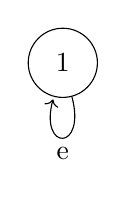
\begin{tikzpicture}
	\node[state]	(1)	{$1$};
	\path[->](1) edge [loop below] node {e} ();
\end{tikzpicture}

We define a functor $\phi = (\mathcal{W}(G), C, \phi_1, \phi_2)$ by $\phi_1(1)
:= A^*$ and $\phi_2(e) := f \circ g \circ h$.

$\phi_2(\mathcal{W}(G))$ is a subcategory of $C$ and it holds:
\[ \phi_2(\mathcal{W}(G))(xyz) = \{ (a^n x b^n y c^n z)\ |\ n \in \mathbb{N} \}
\]

{\bf Example 2}:

We expand on example 1. In addition to $f,g,h$ we have three monoid
homomorphisms $f_1,g_1,h_1$ defined by:
\begin{eqnarray*}
f_1(x) = \epsilon, f_1(u) = u \quad\forall u \in A - \{x\} \\
g_1(y) = \epsilon, g_1(u) = u \quad\forall u \in A - y\} \\
h_1(z) = \epsilon, h_1(u) = u \quad\forall u \in A - z\} \\
\end{eqnarray*}

We extend the graph $G$ as follows to a graph $G_1$:

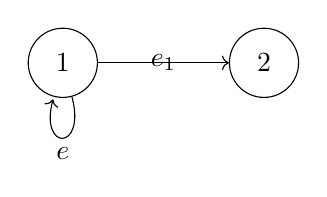
\begin{tikzpicture}
	\node[state] 	(1)										{$1$};
	\node[state] 	(2) [right=60pt]				{$2$};
	\path[->]			(1) edge [loop below] node {$e$} 			()
							 			edge 							node {$e_1$} 	(2);
\end{tikzpicture}

Consider $\mathcal{W}(G_1)(1,2)$. Then $\mathcal{W}(G_1)(1,2) \cup \{1_1,
1_2\}$ is a subcategory of $\mathcal{W}(G_1)$. In addition, $\mathcal{W}(G)$ is
a subcategory of $\mathcal{W}(G_1)$. 

We extend the functor $\phi$ from example 1
onto $\mathcal{W}(G_1)$ by defining:
\[ \phi_2(e_1) := f_1 \circ g_1 \circ h_1 \]

We get:
\[ \phi_2(\mathcal{W}(G_1)(1,2))(xyz) = \{ (a^n b^n c^n\ |\ n \in \mathbb{N} \}.
\]

{\bf Example 3}:

Let $G$ be defined as follows:

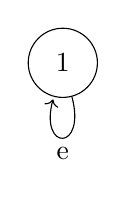
\begin{tikzpicture}
	\node[state]	(1)	{$1$};
	\path[->](1) edge [loop below] node {e} ();
\end{tikzpicture}

The full subcategory of $\mathcal{W}(G)$ generated by $\{ 1', 2', 3' \}$ is the
path category $\mathcal{W}(G')$ with the following graph $G'$:

FIGURE

As an exercise, one can show: The mapping $\phi_1$ defined by 
\begin{eqnarray*}
\phi_1(1) & = & 1' \\
\phi_1(4) & = & 1' \\
\phi_1(2) & = & 2' \\
\phi_1(5) & = & 2' \\
\phi_1(3) & = & 3' \\
\phi_1(6) & = & 3' \\
\end{eqnarray*}
can be extended to a functor $\phi = (\mathcal{W}(G), \mathcal{W'}(G'),
\phi_1, \phi_2)$ where $\phi_2$ has to be chosen in a suitable way.

Remark: The preimage of a closed path does not have to be closed.

We prove now the following
\begin{lemma}
Let \[ C_i = (O_i, M_i, Q, Z, \circ),\ i = 1, 2, 3 \] be categories and $C_1$
and $C_2$ be subcategories of $C_3$. Then $C_1 \cap C_2$ is a category.
\end{lemma}

Proof: It holds
\begin{enumerate}
  \item $w \in O_1 \cap O_2 \Rightarrow 1_w \in M_1 \cap M_2$
  \item $f, g \in M_1 \cap M_2 \Rightarrow f \circ g \in M_1 \cap M_2$, if
  $Z(f) = Q(g)$
\end{enumerate}

It follows that $C_1 \cap C_2$ is a category.

\begin{lemma}
Let $ C_i = (O_i, M_i, Q, Z, \circ),\ i \in I,$\ where $I$ is an arbitrary
index set, be categories. If $C_I, i \in I,$\ are subcategories of a category
$C$, then \[ \tilde{C} := \bigcap_{i \in I} C_i \] is a category.
\end{lemma}

The proof is similar as the one of the previous lemma.

\begin{definition}[generated subcategory]

Let $C = (O, M, Q, Z, \circ)$\ be a category and $O_1 \subset O, M_1 \subset M$
and \[ \mathcal{U}_C(O_1, M_1) := \{ C'\ |\ C'\ \mbox{is subcategory of}\ C, O_1
\subset O', M_1 \subset M' \}. \]

Then \[ {<}O_1, M_1{>} := \bigcap_{C' \in \mathcal{U}_C(O_1, M_1)} C' \] is
called the subcategory of $C$ generated by $(O_1, M_1)$ and $(O_1, M_1)$ is called the
generating system of ${<}(O_1, M_1){>}$.
\end{definition}

Obviously for each category $C = (O, M, Q, Z, \circ)$ it holds: $C = {<}O,
M{}>$.

We say $M_1$ ''generates'' ${<}O_1, M_1{>}$, if \[ O_1 = \{ Q(m)\ |\ m \in M_1
\} \cup \{ Z(M)\ |\ m \in M_1 \}. \]

We have already seen an example for a nontrivial generating system.

Let $G = (V,E)$ be a graph, then $E$ is a generating system of $\mathcal{W}(G)$
which means $\mathcal{W}(G) = {<}E(G){>}$. The path category of a graph has a
special property namely that $E(G)$ is a {\bf free} generating system of
$\mathcal{W}(G)$.

\begin{definition}[free generating system]
Let $C = (O, M, Q, Z, \circ)$ be a category and $E \subset M$. $E$ is called a
{\bf free generating system} of $C$, if the following holds:

If $C' = (O', M', Q, Z, \circ)$ is an arbitrary category and $\phi_1 : O \to O'$
and $\phi_s : E \to M'$ are mappings which fulfill the following diagram:

\begin{center}
\begin{tikzcd}[row sep=large,column sep=huge]
 O \arrow[leftarrow]{r}{Q} \arrow{d}{\phi_1} & E \arrow{r}{Z}
 \arrow{d}{\phi'_2} & O \arrow{d}{\phi_1} \\
 O' \arrow[leftarrow]{r}{Q} & M' \arrow{r}{Z} & O'
\end{tikzcd}
\end{center}

Then there exists a unique continuation of $\phi'_2$ to $\phi_2 : M \to M'$ such
that $\phi = (C, C', \phi_1, \phi_2)$ is a functor.
\end{definition}

\begin{definition}[free category]
A category $C$ is called {\bf free} if there exists a free generating system $E$
of $C$.
\end{definition}

We formulate now our observation above as a theorem:

\begin{theorem}
Let $G = (V, E)$ be a graph. Then $E$ is a free generating system of
$\mathcal{W}(G)$.
\end{theorem} 

Proof: Let $G = (V, E)$ be a graph and $C$ an arbitrary category. Let $\phi_1 :
E \to O,\ \phi'_2 : E \to M$ be mappings and the following diagram commute:

\begin{center}
\begin{tikzcd}[column sep=huge,row sep=large]
 V \arrow[leftarrow]{r}{Q} \arrow{d}{\phi_1} & E \arrow{r}{Z}
 \arrow{d}{\phi'_2} & V \arrow{d}{\phi_1} \\
 O \arrow[leftarrow]{r}{Q} & M \arrow{r}{Z} & O
\end{tikzcd}
\end{center}

We define \[ \phi_2(P,P) = 1_{\phi_1(P)}, P \in V \] and \[ \phi_2(e) =
\phi'_2(e), e \in E \]

Let $\phi_2(w)$ be defined for all $w \in \mathcal{W}(G)$ with $|w| \leq n, n
\geq 1$ and $\phi_2$ be compatible with $Q$ and $Z$ for all these paths $w$.

Further let $\phi_2$ be uniquely determined for these paths $w$ and it holds: \[
\phi_2(w \cdot v) = \phi_2(w) \cdot \phi_2(u) \]
for all $w, v$ with $|w \cdot v| \leq n$.

Now let $v = (P, s_1, \ldots, s_{n+1}, P') \in \mathcal{W}(G)$. We split $v$
into \[ v = (P, \underbrace{s_1, \ldots, s_n}_{v_1}, P'') \cdot (P'',
\underbrace{s_{n+1}}_{v_2}, P') \].

By induction hypothesis, $\phi_2(v_1)$ and $\phi_2(v_2)$ are defined.

For $\phi_2$ to become a functor, necessarily $\phi_2(v) = \phi_2(v1) \cdot
\phi_2(v_2)$ must hold.

By assumption, $\phi_2$ is compatible with source and target mappings $Q$ and
$Z$ for $v_1$ and $v_2$. Therefore $Z(\phi_2(v_1)) = Q(\phi_2(v_2))$ and
$\phi_2(v)$ is defined.

Let $v = u_1 \cdot u_2$ be any partition of $v$, so \[ v = (P, \underbrace{s_1,
\ldots, s_j}_{u_1}, \bar{P}) \cdot (\bar{P}, \underbrace{s_{j+1},
\ldots, s_{n+1}}_{u_2}, P'). \]

By induction hypothesis it holds:
\begin{enumerate}
  \item $Z(\phi_2(u_1)) = Q(\phi_2(u_2))$, so $\phi_2(u1) \cdot \phi_2(u_2)$ is
  defined.
  \item With $u'_2 = (\bar{P}, s_{j+1}, \ldots, s_n, P'')$ we have
  \begin{eqnarray*}
  \phi_2(u_1) \cdot \phi_2(u_2) & = & \phi_2(u_1) \cdot (\phi_2(u'_2) \cdot
  \phi_2(v_2)) \\
  & = & (\phi_2(u_1) \cdot \phi_2(u'_2)) \cdot \phi_2(v_2) \\
  & = & \phi_2(v_1) \cdot \phi_2(v_2) \\
  & = & \phi_2(v)
  \end{eqnarray*}
\end{enumerate}

It remains to show \[ \phi_1(Q(v)) = Q(\phi_2(v)),\quad \phi_1(Z(v)) =
Z(\phi_2(v)) \]

This follows directly from $Q(v) = Q(v_1)$ and $Z(v) = Z(v_2)$ by induction
hypothesis.

\begin{theorem}
To each category $C$ there exists a free category $F$ and a surjective functor
$\phi = (F, C, \phi_1, \phi_2)$.
\end{theorem}

Proof: For the category $C$, create the oriented graph $G_C = (V, E)$ with $V =
Obj(C)$ and $E = \{ f\ |\ Q(f) = O_1, Z(f) = O_2, f : O_1 \to O_2 \in M \}$.

That means: The objects of the category become the points of the graph and each
morphism becomes an edge between the corresponding source and target objects.
Because $\mathcal{W}(G_C)$ is a free category by theorem 1 we can choose $F$ to
be exactly this category.

Let $\phi_1 : V \to O$ with $\phi_1(w) = w$ and $\phi'_2 : E \to M$ with
$\phi'_2(f) = f$ be mappings and $\phi_2 : \mathcal{W}(G_C) \to M$ be the
continuation of $\phi'_2$ such that $\phi = (\mathcal{W}(G_C), C, \phi_2,
\phi_2)$ becomes a functor.

By construction, $\phi$ is surjective.

The following theorem tells about the uniqueness of free generating systems.

\begin{theorem}
If $E$ and $E'$ are free generating systems of a category $F$, then $E = E'$.
\end{theorem}

The proof is similar to the one of the corresponding theorem for free monoids.

\section{Grammars and derivations}

In the introduction of this book we already learned about formal languages. The
wish to describe these in general infinite sets of words by a finite generating
system leads to the notion of a {\bf grammar}.

\begin{definition}[Chomsky grammar]
$G = (N, T, P, s)$ is a {\bf Chomsky grammar}, if
\begin{enumerate}
  \item $N$ is a finite, nonempty set of {\bf nonterminal symbols}
  \item $T$ is a finite, nonempty set of {\bf terminal symbols} with
  $N \cap T = \emptyset$
  \item $P \subset N^+ \times (N \cup T)^*$ is a finite set of {\bf productions}
  \item $S \in N$ is the {\bf axiom} or {\bf start symbol} 
\end{enumerate}
\end{definition}

Notation: For $p = (u, v) \in P$ we also write $u \stackrel{p}{\to} v$ and
$Q(p) = u, Z(p) = v$ denote the source and target of a production.

Examples:
\begin{enumerate}
  \item $G_1 = (N, T, P, S)$ with $N = \{ S \}, T = \{ x, x' \},$ \\ 
  $P = \{ S \to SS, S \to xSx', S \to \epsilon \}$
  \item $G_2 = (N, T, P, S)$ with $N = \{ S, X \}, T = \{ x, x' \}$ \\
  $P = \{ S \to xSX, S \to xX, X \to x'S, X \to x' \}$
\end{enumerate}

To use a grammar for generating the words of a language, starting with the axiom
there are intermediate words generated by application of the productions, until
the produced word will contain terminal symbols only. This leads to the notation
of a ''derivation'' which we will now define formally.

\begin{definition}[directly derivable, derivable]
Let $G = (N, T, P, S)$ be a grammar and let $w, w' \in (N \cup T)^*$.

$w'$ is {\bf directly derivable} from $w$ in $G$, notation: $w
\dderives{G} w'$, if there are segmentations $w = w_1 \cdot u \cdot w_2$ and
$w' = w_1 \cdot v \cdot w_1$ and a production $(u, v) \in P$.

$w'$ is {\bf derivable} from $w$, notation: $w \derives{G} w'$, if there exists
a sequence of words \[ w = w_0, \ldots, w_n = w',\quad n \in \mathbb{N}, w_i \in
(N \cup T)^* \] such that for each $0 \leq i \leq n : w_i \dderives{G}
w_{i+1}$.
\end{definition}

Such a sequence is called a {\bf derivation} of length $n$. $Q$ and $Z$ can be
extended in a natural way to derivations.

A derivation is called {\bf canonic} or {\bf leftmost}, if in each step $w
\dderives{G} w'$ it holds:

If $w = w_1 \cdot u \cdot w_2$ and $w' = w_1 \cdot v \cdot w_2$ are the
segmentations and $(u, v) \in P$ the applied production, then $w_1 \in T^*$
which means that always the leftmost nonterminal is replaced.

If the grammar is known we omit the index $G$ from the symbols $\dderives{G}$
and $\derives{G}$.

Let us consider some properties of the relation $\derives{G}$:

\begin{lemma}
Let $G$ be a grammar. Then the following holds:
\begin{enumerate}
  \item $(u, v) \in P \Rightarrow u \derives{G} v$
  \item $w \derives{G} w$ (reflexivity)
  \item $w \derives{G} w' \wedge w' \derives{G} w'' \Rightarrow w \derives{G}
  w''$ (transitivity)
  \item $w_1 \derives{G} w'_1 \wedge w_2 \derives{G} w'_2 \Rightarrow w_1 \cdot
  w_2 \derives{G} w'_1 \cdot w'_2$ (compatibility with monoid operation)
\end{enumerate}
Here $w, w', w'', w_1, w_2, w'_1, w'_2 \in (N \cup T)^*$.
\end{lemma}

Proof:
\begin{enumerate}
  \item follows from the definition of $\derives{G}$.
  \item clear with $n = 0$ in the definition of $\derives{G}$.
  \item There exist sequences $w = w_0, \ldots, w_n = w',\ w' = w'_0, \ldots,
  w'_m = w''$ with $w_i \derives{G} w_{i+1}$ and $w'_j \derives{G} w'_{j+1}$.
  Because $w_n = w' = w'_0$, the composed sequence $w = w_0, \cdots, w_n, w'_1,
  \cdots, w'_n = w''$ is a derivation from $w$ to $w''$.
  \item Exercise for the reader
\end{enumerate}

Notation: An intermediate word that is generated by a derivation starting with
the axiom is called a {\bf sentence form} of $G$. We define:

\begin{definition}
\[ SF(G) := \{ w \in (N \cup T)^*\ |\ S \derives{G} w \} \] is the set of {\bf
sentence forms} of $G$.
\end{definition}

Now we are able to define the formal language generated by a grammar.

\begin{definition}
Let $G = (N, T, P, S)$ be a grammar. \[ L(G) := \{ w \in T^*\ |\ S \derives{G} w
\} \] is the {\bf language generated by} $G$.
\end{definition}

Note: $L(G) = SF(G) \cap T^*$.

Examples:
\begin{enumerate}
  \item One can see that for the grammar $G_1$ given in the previous example 1
  it holds: $L(G_1)$ is the Dyck language over the alphabet $\{ x, x' \}$.
  \item Let $G = (N, T, P, S)$ with $N = \{ S \}, T = \{ a, b \}, P = \{ S \to
  aSb, S \to \epsilon \}$. Then $L(G) = \{ a^n b^n \ |\ n \in \mathbb{N}$.
\end{enumerate}

The simple proof is left to the reader.

Grammars are compared with relation to the languages they generate. We define:

\begin{definition}[weak grammar equivalence]
$G$ is {\bf weakly equivalent} to $G' \Leftrightarrow L(G) = L(G')$.
\end{definition}

Remark: The reader should convince himself that the grammars $G_1$ and $G_2$
from the first example generate the same language.

Of course you can define infinitely many different grammars for each language.

We now can define different classes of grammars (and languages generated by
these) depending on certain restrictions of their production system. In the next
chapter we will meet the so called {\em right-linear} grammars and their
languages.

Special importance, also from a practical point of view, have the so called
{\em contextfree} grammars.

\begin{definition}[context-free grammar]
A grammar $G = (N, T, P, S)$ is called {\bf context-free} if $P \subset N \times
(N \cup T)^*$.
\end{definition}

The term ''context-free'' describes the fact that in a sentence-form a
nonterminal may be replaced by the right-hand side of a production without need
to respect the ''context'' to the left and right around that nonterminal symbol.

In chapter 4 we will treat context-free grammars in depth.






























\chapter{Finite Automata}
\section{The finite automaton, regular sets in $X^*$,\ $REG(X^*)$}

Let $G = (V, E)$ be a finite, oriented graph, $X$ a finite set and $\alpha =
(\pathcat{G}, X^*,\alpha_1, \alpha_2)$ a functor with $\alpha_1 : V \to \{ X^*
\},\ \alpha_2 : \pathcat{G} \to X^*$.

(Remark by the translator: Here the free monoid $X^*$ is regarded as a category
$X^* = (\{X^*\}, X^*, Q, Z, \cdot \})$ where $\cdot$ is the monoid operation
(word concatenation). Words are treated as morphisms with source and target
$X^*$. Klingt komisch, is aber so.)

\begin{definition}[nondeterministic finite automaton]
$\fa{A} = (G, X^*, \alpha)$ is called a {\bf nondeterministic finite
automaton}.
\end{definition}

If $S, F \in V$ are points of the graph $G$, we call $\fa{A} = (G, X^*,
S, F, \alpha)$ a finite automaton with start and final states or shortly a {\bf
finite acceptor}.

In the following we will use the terms acceptor and automaton as synonyms.

If the finite automaton works over the free monoid $X^*$ we write shorter just
$X$ instead of $X^*$, otherwise we specify the monoid explicitly.

\begin{definition}[accepted set]
If we define 
\[ \pathcat{G}(S, F) := \{ w \in \pathcat{G}\ |\ Q(w) \in S \wedge Z(w)
\in F \}, \]
then \[ L_{\fa{A}} := \alpha_2(\pathcat{G}(S, F)) \] 
is called the set {\bf accepted by} the automaton. 
\end{definition}

We will also write shortly $\alpha$ instead of $\alpha_2$ and $\pathcat{}(S,F)$
instead of $\pathcat{G}(S,F)$.

\begin{definition}[regular language over free monoid]
Let $X$ be an alphabet. \[ REG(X^*) := \{ L \subset X^*\ | \mbox{ there
exists a finite automaton } \fa{A} \mbox{ with } L = \lang{A} \}
\]

$REG(X^*)$ is the set of {\bf regular languages} over the free monoid $X^*$.
\end{definition}

Remark: We defined here the finite automaton via its ''state graph''. Most
often, the definition is given using the ''next state relation'' as follows:

\[ \delta = \{ (a, P_1, P_2) \in X \times V \times V)\ | \]
\[ \mbox{there exists an edge } e \mbox{ with } Q(e) = P_1, Z(e) = P_2 \mbox{
and } \alpha(e) = a \in X \}. \]

$\delta$ my be regarded as a relation between $X \times V$ and $V$ where $X$ is
the input alphabet and $V$ the state set of the automaton \[ \fa{B} = (X,
V, \delta, S, F) \]

The elements of $V$ denote the current state of the automaton $\fa{B}$.

If the automaton $\fa{B}$ is in state $z \in V$ and reads the symbol $x
\in X$ then it changes into state $z' \in V$ where $(x, z, z') \in \delta$. If
there doesn't exist such a $z'$ the automaton halts.

This interpretation can be visualized as follows:

FIGURE

Let's return to out definition of the finite automaton. We explain its
working based on our definition:

The automaton $\fa{A} = (G, X, S, F, \alpha)$ may be interpreted as a
nondeterministic algorithm. The points of graph $G$ define the possible states
of the algorithm, the elements of $X$ are the input alphabet.

The nondeterministic automaton $\fa{A}$ which reads a symbol $x \in X$
while in state $P \in V$ changes into state $P'$ if there exists an edge $e$
from $P$ to $P'$ with label $\alpha(e) = x$. If the graph has no such edge
originating in $P$ the automaton is set ''out of service''.

A finite acceptor accepts a word $w \in X^*$ if there exists a path from a point
in $S$ to a point in $F$ which is labeld with $w$.

Let's consider some examples for finite automata:

Example 1: Let $X = \{ a, b \}$ and $L = \{ (a b)^{2n}\ |\ n \in \mathbb{N} \}$.
It holds: $L \in REG(\{a, b\}^*)$.

The following acceptor accepts $L$ (exercise):

$\fa{A} = (G, \{a, b\}, {1}, {1}, \alpha)$.

FIGURE

Example 2: Lexical analysis, check for special characters.

In every programming language there exist special character combinations
(reserved words) that mark certain program actions. These have to be identified
during the lexical analysis. We give a finite acceptor which realizes such a check for a selection
of reserved words:

Let the set of reserved words be 
$\{$ 'BEGIN', 'END', 'ELSE', 'IF', FI', 'FOR', 'INTEGER', 'THEN', 'LOOP',
'POOL', 'PROCEDURE' $\}$.

The following acceptor accepts this set:

FIGURE

The images of the edges under the mapping $\alpha$ are shown as edge labels. The
points of the graph are the ovals with their labels. Start and final states are
given by $S = \{$ START $\}$ and $F = \{$ STOP $\}$.

The labels of the points are chosen such that one can see the information stored
by the automaton.

Now we want to prove some properties of $REG(X^*)$. To do that, we need
some basic properties for finite automata.

\begin{lemma}
Let $\fa{A} = (G, X, S, F, \alpha)$ be a finite automaton. Then there
exists a finite automaton $\fa{A'} = (G', X, S', F', \alpha')$ such that
$card(S') = card(F') = 1$ and $\lang{A} = \lang{A'}$.
\end{lemma}

An automaton with a single start state is called {\bf initial}.

Proof: If $card(S) = card(F) = 1$ we are done.

(Comment by translator: The proof in the book is completely unreadable because
of all these tildes, primes, indices etc. Therefore it is reformulated here.) 

Let $card(S) > 1$ or $card(F) > 1$.

1. Add new edges leaving the new start state $S'$:

Define the set of all edges leaving an old start state by
\[ OUT := \{ e \in E \mid Q(e) \in S \} \]
Add the following new edges to the graph:
\[ OUT' := \{ e' = (S', Z(e)) \mid e \in OUT,\ \alpha'(e') := \alpha(e) \} \]

2. Add new edges reaching the new final state $F'$:

Define the set of all edges reaching an old final state by
\[ IN := \{ e \in E \mid Z(e) \in F \} \]
Add the following new edges to the graph:
\[ IN' := \{ e' = (Q(e), F') \mid e \in IN,\ \alpha'(e') := \alpha(e) \} \]

To each new edge we assign the same label as the edge from which it has been
derived.

The new automaton $\fa{A'} = (G', X, \{S'\}, \{F'\}, \alpha')$ is defined
by the graph $G' = (V \cup \{ S', F' \}, E \cup OUT' \cup IN')$
and the new labeling $\alpha'$ which is identical to $\alpha$ for all existing edges and is defined as shown above for the new edges.

It is easily shown that $\lang{A'} = \lang{A}$.

\begin{lemma}
Let $\fa{A} = (G, X, S, F, \alpha)$ be a finite automaton. Then there
exists an automaton $\fa{A'} = (G', X, S', F', \alpha')$ with $\alpha'(e)
\in X\ \forall e \in E(G)$ and $\lang{A} = \lang{A'}$.
\end{lemma}

Proof: We ''split'' all edges according to their labels.

\begin{enumerate}
  \item Let $e \in E$ with $\alpha_2(e) = x_1 \cdots x_k,\ k > 1, x_i \in X$.\\
  Remove edge $e$ and add new edges $e'_1,
  \ldots, e'_k$ and new points $P'_1, \ldots, P'_{k-1}$ such that $(Q(e),
  e'_1, \ldots, e'_k, Z(e)) \in \pathcat{G'}$ and define a new graph $G' =
  (V', E')$. The labeling of the new edges is defined by $\alpha'(e'_i) := x_i$
  for $i = 1, \ldots, k$.
  
  Then $\alpha_2(e) = \alpha'_2(e'_1) \cdots \alpha'_2(e'_k)$.
  
  \item Let $e \in E$ be an edge labeled with $\epsilon$.
  \begin{enumerate}
    \item  (Remove $\epsilon$-loops) \\
    If $Q(e) = Z(e) : E' := E - e$
    \item (Remove
    $\epsilon$-edges which cannot be continued to a longer path)\\
    If there is
    not $e' \in E$ with $Q(e') = Z(e') : E' := E - e$
    \item  (Skip $\epsilon$-edges that can be continued and remove the
    $\epsilon$-edge)\\
    If there exists an edge $e' \in E$ with $Q(e') = Z(e) : E'' := E - e$.
    Add new edges: $E' := E'' \cup \{
    \tilde{e} \mid Q(\tilde{e}) = Q(e), Z(\tilde{e}) = Z(e'),\
    alpha'(\tilde{e}) := \alpha(e') \}$
  \end{enumerate}
  If in step (b) or (c) the target of the edge is a final state, then add the
  source of the edge to the set of final states.
  
  Continue this algorithm inductively until no more $\epsilon$-edges remain in
  the graph. The algorithm terminates because the point and edge sets are
  finite. For the new automaton $\fa{A'}$ that results from this algorithm
  holds: $\lang{A'} = \lang{A}$.
\end{enumerate}

If we apply this algorithm to our automaton from example 1, we obtain:

FIGURE

Now we want to prove some closure properties of $REG(X^*)$.

\begin{theorem}[Regular languages are closed under union and intersection]
\[ L, L' \in REG(X^*) \Rightarrow L \cup L' \in REG(X^*) \wedge L \cap L' \in
REG(X^*) \]
\end{theorem}

Proof: Let $L = \lang{A}$ and $L' = \lang{B}$ with automata \[
\fa{A} = (G_A, X, S_A, F_A, \alpha) \] and \[ \fa{B} = (G_B, X, S_B,
F_B, \beta).\]
We may assume that the edge and point sets of both automata graphs are disjoint.

\begin{enumerate}
  \item Closure under union: Define
	\[ \gamma_2(e) := \left\{
		\begin{array}{l} 
		\alpha_2(e),\ e \in E(G_A) \\
		\beta_2(e),\ e \in E(G_B)
		\end{array}
	 \right. \]

	Then the automaton $\fa{C} = (G_A \cup G_B, X, S_A \cup S_B, F_A \cup
	F_B, \gamma)$ accepts the language $\lang{A} \cup \lang{B}$.
	
	\item Closure under intersection: Define $G' = (V', E')$ where
	\[ V' = V_A \times V_B \]
	\[ E' = \{ (e_A, e_B) \in E_A \times E_B \mid \alpha_2(e_A) = \beta_2(e_B)
		 \}. \]
	By lemma 2 we may assume that the edge labels are all single symbols from $X$.
	
	We define the new labeling $\delta_2$ by \[ \delta_2 : E' \to X,\
	\delta_2((e_A, e_B) = \alpha_2(e_A)). \]
	
	For the automaton $\fa{A'} = (G', X, S_A \times S_B, F_A \times F_B,
	\delta)$ then holds: $\lang{G'} = \lang{A} \cap \lang{B}$
	and this automaton is called the {\bf cartesian product} of $\fa{A}$ and
	$\fa{B}$.
\end{enumerate}

\begin{theorem}[Regular languages are closed under mirror operation]
\[ L \in REG(X^*) \Rightarrow L^R \in REG(X^*) \]
\end{theorem}

Proof: Let $\fa{A} = (G, X, S_{\fa{A}}, F_{\fa{A}}, \alpha)$ be a
finite acceptor for $L$.

Create the graph $G' = (V(G), E')$ where $E'$ is a set with the same cardinality
as $E$. There exists a bijection from $E$ to $E'$ mapping edges as follows:
\[ e : P \to P' \in E \Leftrightarrow e' : P' \to P \in E' \]
which means we reverse the orientation of the edges.

For the resulting automaton $\fa{A'} = (G', X, S_{\fa{A}},
F_{\fa{A}}, \alpha')$ with $\alpha'(e') = \alpha(e)$ for all edges of $G'$
it holds: $\lang{A'} = \lang{A}^R = L^R \in REG(X^*)$.

\begin{definition}[deterministic and complete automaton]
Let $\fa{A} = (G, X, S, F, \alpha)$ be a finite automaton with
$\alpha(E(G)) \subset X$ (each edge is labeled with a single
symbol).

$\fa{A}$ is called {\bf deterministic} $\Leftrightarrow$ for all $e, e'
\in E(G)$ with $Q(e) = Q(e')$ and $\alpha(e) = \alpha(e')$ it holds: $e$ = $e'$.

$\fa{A}$ is called {\bf complete} $\Leftrightarrow$ for each $P \in V(G)$
and $x \in X$ there exists an edge $e \in E(G)$ with $Q(e) = P$ and $\alpha(e)
= x$.
\end{definition}

\begin{theorem}[Existence of complete, deterministic acceptor]
If \fa{A} is a finite automaton, then there exists a complete,
deterministic automaton \fa{A'} which accepts the same language.
\end{theorem}

Proof: From our lemmata we may assume that $card(S_{\fa{A}}) = 1$ and
$\alpha_2(e) \in X$ for all edges $e$ in the graph of \fa{A}.

We construct an automaton \fa{A'} as follows (''subset construction''):

Instead of the points of the graph $G$ our new graph has the power set
$Pot(V(G))$ of $V(G)$ as its point set.

For $\tilde{P} \in Pot(V(G))$ we define 
\begin{eqnarray*}
& N(x, \tilde{P}) := & \{ P \in V(G) \mid \mbox{there exists an edge } e \in
E(G) \mbox{ with } \\
& & \ Q(e) \in \tilde{P}, Z(e) = \tilde{P} \mbox{ and } \alpha(e) = x \} 
\end{eqnarray*}

The empty set $\emptyset$ is also an element of the power set such that it will
also become a point of the new graph.

Let $\tilde{P}, \tilde{R} \in Pot(V(G))$. These points are connected by an edge
$e$ with label $\alpha'_s(e) = x \Leftrightarrow \tilde{R} = N(x, \tilde{P})$.

This defines our new graph $G' = (V', E')$.

The start and final states are defined as follows:
\[ S_{\fa{A'}} = \{ S_{\fa{A}} \} \]
\[ F_{\fa{A'}} = \{ \tilde{R} \in Pot(V(G)) \mid \tilde{R} \cap
F_{\fa{A}} \neq \emptyset \} \]

This completes the definition of automaton $\fa{A'} = (G', X,
S_{\fa{A'}}, F_{\fa{A'}}, \alpha')$.

We first prove that
\fa{A'} is complete and deterministic:

\fa{A'} has a single start state $S_{\fa{A'}} = \{ S_{\fa{A}}
\}$, the edge labels are all single symbols and 
\[ card(\{ e \in E' \mid Q(e) = \tilde{P}, \alpha'_2(e) = x \}) = 1 \]
for all $\tilde{P} \in V(G')$.

Now we prove that the accepted languages are equal:

''$\subset$'': We use diagrams of the following form:
\begin{eqnarray*}
& P \edge{x} R & \\
& \tilde{P} \edge{x} \tilde{R} &
\end{eqnarray*}

which are to be understood as follows: For $P \edge{x} R \in E(G)$
there exists by construction $\tilde{P} \edge{x} \tilde{R} \in
E(G')$ with $P \in \tilde{P}$ and $R \in \tilde{R}$.

Starting with $S_{\fa{A'}} = \{ S_{\fa{A}} \} = \{ \{ P_0 \} \}$ and
concatenating these diagrams, we get for $x_1 \cdots x_k \in
L_{\fa{A}}$:
\begin{eqnarray*}
 & & P_0 \edge{x_1} P_1 \edge{x_2} P_2 \edge{} \ldots \edge{} P_{k-1} \edge{x_k}
 P_k \in F_{\fa{A}} \\
 & & \tilde{P}_0 \edge{x_1} \tilde{P}_1 \edge{x_2} \tilde{P}_2 \edge{} \ldots
 \edge{} \tilde{P}_{k-1} \edge{x_k} \tilde{P_k}
\end{eqnarray*}

That means $\tilde{P_k} \cap F_{\fa{A}} \neq \emptyset \Rightarrow \tilde{P}_k \
\in F_{\fa{A'}} \Rightarrow w \in \lang{A'}.$

\[ \Rightarrow \lang{A} \subset \lang{A'}\]

''$\supset$'': Here we use diagrams  
\begin{eqnarray*}
& \tilde{P} \edge{x} \tilde{R} & \\
& P \edge{x} R & 
\end{eqnarray*}

which are to be understood as follows: For $\tilde{P} \edge{x} \tilde{R} \in
E(G')$ and $R \in \tilde{R}$ there exists $P \in \tilde{P}$ with $P \edge{x} R
\in E(G)$.

For $x_1 \cdots x_K \in \lang{A'}$ we start with $F_{\fa{A'}}$ and continue
the diagram from right to left. For $P_k \in \tilde{P}_k \cap F_{\fa{A}}$ we get
\begin{eqnarray*}
 & S_{\fa{A'}} \ni & \tilde{P}_0 \edge{x_1} \tilde{P}_1 \edge{x_2} \tilde{P}_2 \edge{} \ldots
 \edge{} \tilde{P}_{k-1} \edge{x_k} \tilde{P_k} \in F_{\fa{A'}} \\
 & & P_0 \edge{x_1} P_1 \edge{x_2} P_2 \edge{} \ldots \edge{}
 P_{k-1} \edge{x_k} P_k \in F_{\fa{A}} 
\end{eqnarray*}

Because of $S_{\fa{A'}} = \{ S_{\fa{A}} \} = \{\{ P_0 \}\}$ it holds: $x_1
\cdots x_k \in \lang{A} \Rightarrow \lang{A'} \subset \lang{A}$.

\[ \Rightarrow \lang{A'} \subset \lang{A}\]

From both inclusions we get $\lang{A} = \lang{A'}$.

Remark: The state set grows exponentially when the automaton is made
deterministic. The following example will clarify this fact \cite{Co}.

Example: Let $X = \{ a, b \}$. Define for arbitrary, but fixed $n \in
\mathbb{N}$ \[ L_n := \{ w \mid w = w_1 \cdot w_2 \mbox{ with } w1 \neq w_2, |w_1| = |w_2|
= n, w_1, w_2 \in X^* \} \]

$L_n \in REG(X^*)$ because there exists a nondeterministic finite acceptor
$\fa{A}_{n}$ with $L_n = L_{\fa{A}_{n}}$.

We want to give the automaton for $n = 3$:

$\fa{A}_3 = (G_3, \{a,b\}, \{1\}, \{22\}, \alpha)$ with the following graph
$G_3$:

FIGURE

The labeling $\alpha$ is shown at the edges.

Exercise: Show that this automaton accepts $L_3$.

If we construct for $L_3$ from the nondeterministic acceptor $\fa{A}_3$
the deterministic acceptor $\fa{A'}_3$, the graph $G'_3$ looks as follows:

FIGURE

The edges pointing upwards are labeled with $a$ and the edges pointing downwards
with $b$.

$G'_3$ is the graph of the complete (up to loops in the final state and state
$\emptyset$), deterministic acceptor $\fa{A'}_3$ and accepts the language $L_3$
(exercise).

In \cite{Co} it is proved that this automaton is minimal in the number of
states.

Making a state graph deterministic brings advantages as well as disadvantages. A
program simulating finite automata based on the given state graph is fast for
a deterministic graph. However it needs more space because of the possibly very
large representation of the deterministic graph.

If the program uses the nondeterministic graph, it can follow all alternatives
in parallel similar to our construction of the deterministic automaton. It needs
less memory but the computing time can grow linear for each simulation step.

We want to state an important consequence from our last theorem.

\begin{theorem}[Regular languages are closed under complement]
\[ L \in REG(X^*) \Rightarrow \bar{L} = X^* - L \in REG(X^*) \]
\end{theorem}

Proof: 

$L \in REG(X^*) \Rightarrow $ there exists a complete, deterministic
finite acceptor $\fa{A}$ with $\lang{A} = L$.

Define $\fa{A'} = (G, X, S_{\fa{A}}, F_{\fa{A}}, \alpha)$ where $F_{\fa{A}} :=
V(G) - F_{\fa{A}}$.

Because \fa{A} is complete and deterministic, every word $w \in X^*$ determines
a unique path starting in $S_{\fa{A}}$.

This $w \in X^*$ uniquely determines a point $P \in V(G)$ with $w \in
\alpha(\pathcat{W}(S_{\fa{A}}, P))$.

It is either $P \in F_{\fa{A}}$ or $P \in F_{\fa{A'}}$ and from $F_{\fa{A}}
\cap F_{\fa{A}'} = \emptyset$ follows $w \in \lang{A} \Leftrightarrow w
\notin \lang{A'}$ and therefore $\lang{A'} = \bar{\lang{A}}$.

\begin{theorem}[Regular languages are closed under concatenation]
\[ L_1, L_2 \in REG(X^*) \Rightarrow L_1 \cdot L_2 \in REG(X^*) \]
\end{theorem}

Proof: $L_1, L_2 \in REG(X^*) \Rightarrow$\ there exist finite acceptors
$\fa{A}_i = (G_i, X, S_i, F_i, \alpha_i)$ with $L_i = \lang{A}_i,\ i = 1,2$.

We define a new acceptor
\[\fa{A} = (G, X, S, F, \alpha) \]
as follows:

Vertices:
\[ V(G) := V(G_{\fa{A}_1}) \cup V(G_{\fa{A}_2})\mbox{ where }V(G_{\fa{A}_1})
\cap V(G_{\fa{A}_2}) = \emptyset \]

Edges:
\[ E(G) = E(G_{\fa{A}_1}) \cup E(G_{\fa{A}_2}) \cup \mbox{ 'bridge'' edges
defined as follows:}
\]

FIGURE (bridge edge)

Here $R \in F1$ is a final state in $\fa{A}_1$, $x = \alpha_1(e_1)$ is the label
of edge $e_1$, $P'$ is a start state in $\fa{A}_2$.

For each such configuration, a new ''bridge''	edge $e$ is added to $E(G)$ where
\[ Q(e) := P,\ Z(e) := P' \mbox{ and } \alpha(e) := x.\]

Start and final states: $S := S_{\fa{A}_1}$ and $F := F_{\fa{A}_2}$.

We now prove that $\lang{A} = \lang{A}_1 \cdot \lang{A}_2$.

\begin{enumerate}
  \item $\lang{A} \supset \lang{A}_1 \cdot \lang{A}_2$
  
  Let $u = u_1 \cdots u_n \in \lang{A}_1$ and $v = v_1 \cdots v_m \in
  \lang{A}_2$. Then there exist accepting paths
  \[ S_1 \ni P_0 \edge{u_1} P_1 \edge{u_2} \ldots \edge{u_n} P_n \in F_1 \]
  and 
  \[ S_2 \ni Q_0 \edge{v_1} Q_1 \edge{v_2} \ldots \edge{v_m} Q_m \in F_2 \]
  
  By construction of graph $G$ there exists a path in $\pathcat{G}(S1, F2)$ of
  the form
  \[ S_1 \ni P_0 \edge{u_1} P_1 \edge{u_2} \ldots P_{n-1} \edge{u_n} Q_0
  \edge{v_1} Q_1 \edge{v_2} \ldots \edge{v_m} Q_m \in F_2 \]
  
  It follows $u = u_1 \cdots u_n \cdot v_1 \cdots v_m \in \lang{A}$ thus
  $\lang{A}_1 \cdot \lang{A}_2 \subset \lang{A}$.
  
  \item $\lang{A} \subset \lang{A}_1 \cdot \lang{A}_2$
  
  Let \[ S \ni P_0 \edge{w_1} P_1 \edge{w_2} \ldots \edge{w_n} P_n \in F \] be
  an accepting path in $\pathcat{G}(S, F)$. Then there exist states $P_i \in
  S_2$ and $P_j \in V(G_1)$ with $j < i$ because $V(G_1) \cap V(G_2) =
  \emptyset$.
  
  FIGURE
  
  Therefore the subpath \[ S_2 \ni P_i \edge{w_{i+1}} P_{i+1} \edge{} \ldots
  \edge{w_n} P_n \in F_2 \] contains only edges and vertices from $\fa{A}_2$ and
  is an accepting path for the word $w_{i+1} \cdots w_n \in \lang{A}_2$.
  
  It holds $P_{i-1} \in V_1$ and by construction of the graph $G$ there exists
  an edge labeled with $w_i$ which ends in a final state of $\fa{A}_1$. So $w_1
  \cdots w_i \in \lang{A}_1$.
  
  Together we get \[ w_1 \cdots w_i \cdots w_n \in \lang{A}_1 \cdot
  \lang{A}_2 \Rightarrow \lang{A} \subset \lang{A}_1 \cdot \lang{A}_2.\]
\end{enumerate}

From (1) and (2) it follows $\lang{A} = \lang{A}_1 \cdot
\lang{A}_2$.

\begin{theorem}[Regular languages are closed under Kleene-star]
\[ L \in REG(X^*) \Rightarrow L^* \in REG(X^*) \]
\end{theorem}

FIGURE (graph construction)

Let $\fa{A} = (G, X, S, F, \alpha)$	be a finite acceptor for $L$, create the
finite acceptor $\fa{A'} = (G', X, S, F, \alpha')$ as follows:

Graph: Take the graph $G$ and add the following edges: 

\begin{enumerate}
  \item For each edge \[e : P \edge{x} R \in E(G),\ R \in F\] leading to a
  final state and each start state $P_0$ add an edge \[e' : P \edge{x} P_0 \]
  labeled by $\alpha'(e') := x$.
  \item For each state $P_0 \in S$ and each final state $R \in F$ add an edge
  (if not already existing) \[ e' : P_0 \edge{\epsilon} R \]
  labeled by $\alpha'(e') := \epsilon$.
\end{enumerate}

For the finite acceptor $\fa{A'}$ it holds (exercise): \[ \lang{A'} = L^* \]

We have seen (lemma 1) that for nondeterministic automata a single start and a
single final state are sufficient, but in the deterministic case, a single final
state in insufficient in general.

\begin{theorem}[Regular languages are closed under homomorphism]
\[ L \in REG(X^*), \phi : X^* \to Y^* \mbox{ monoid homomorphism } \Rightarrow
\]
\[ \phi(L) := \{ \phi(w) \mid w \in L \} \in REG(X^*) \]
\end{theorem}

Proof: Let $\fa{A} = (G, X, S, F, \alpha)$ be a finite acceptor for $L$. Then \[
\fa{B} = (G, Y, S, F, \beta)\] with $\beta_2(e) := \phi(\alpha_2(e)),\ e \in
E(G)$, is an acceptor for $\phi(L)$ because \[\phi(L) =
\phi(\alpha_2(\pathcat{G}(S, F))) = \beta_2(\pathcat{G}(S,F))\]
Therefore \[ \phi(L) \in REG(Y^*) \]

After having proved closure properties, we prove some other important properties
of regular sets.

\begin{lemma}
For $x \in X$ it holds $\{ x \} \in REG(X^*)$ and $\emptyset \in REG(X^*)$.
\end{lemma}

Proof: Set $G = (\{S,F\}, \{e\})$ be a graph, then the finite acceptor
\[\fa{A}_x = (G, \{x\}, \{S\}, \{F\}, \alpha)\] with $\alpha_2(e) = x$ fulfills
$\lang{A} = \{x\}$.

Set $G = (\{S,F\}, \emptyset)$, then $\fa{A} = (G, \emptyset, \{S\}, \{F\},
\emptyset)$ fulfills $\lang{A} = \emptyset$.

\begin{lemma}
Set $G = (V, E)$. Then $\pathcat{G}(S,F) \in REG(E^*)$.
\end{lemma}

This means the set of paths of a graph which start in a start state and end in a
final state is a regular set over the set of edges of the graph. The proof is
trivial, just label the edges with their name.

\begin{definition}[local set]
Let $S, F \subset X$ and $R \subset X \times X$ be a relation on $X$ with \[ L =
\{ x_1 \cdots x_k \mid x_1 \in S, x_k \in F, (x_i, x_{i+1}) \in R,\ i = 1,
\ldots, k - 1 \} \]
\end{definition}

\begin{lemma}[The accepting path set of a FA is local]
Let $G = (V, E)$ be a graph. Then $\pathcat{G}(S, F)$ is local over $E$.
\end{lemma}

Proof: Let \begin{eqnarray*}
S & = & \{ e \in E \mid Q(e) \in S \} \\ 
F & = & \{ e \in E \mid Z(e) \in F \} \\
R & = & \{ (e, e') \in E \times E \mid Z(e) = Q(e') \} 
\end{eqnarray*}

Then the claim is immediately proved.

\begin{lemma}[local sets are regular]
\[ L \mbox{ local over } X \Rightarrow L \in REG(X^*) \]
\end{lemma}

Proof: Let $S$ and $F$ be the subsets of $X$ from the definition of a local
set. We define a graph $G = (V, E)$ as follows:
\begin{eqnarray*}
V & = & X \cup \{ \bar{S} \} \mbox{ with } X \cap \{ \bar{S} \} = \emptyset \\
E & = & \{ e : \{ \bar{S} \} \to x \mid x \in S \} \cup \{ e : x \to y \mid
(x, y) \in R \}
\end{eqnarray*}

Consider the finite acceptor $\fa{A} = (G, X, \{\bar{X}\}, F, \alpha)$ with
labeling $\alpha$ defined by $\alpha_2(e) = Z(e)$ for each edge $e \in E$.

Then it is clear that $\lang{A} = L$.

\begin{lemma}[Each regular set is homomorphic image of a local set]
$L \in REG(X^*)$, then there exists a local set $R$ over $X$ and a monoid
homomorphism $\phi$ such that \[ \phi(R) = L \]
\end{lemma}

Proof: Exercise

We want to summarize our results to some main theorems where we organize these
results differently.

Let $X_\infty = \{ x_1, x_2, \ldots \}$ be an infinite alphabet. Define \[
REG(X_\infty^*) = \bigcup_{X	\subset X_\infty} REG(X^*), \mbox{$X$ is finite}
\]

\begin{maintheorem}
\begin{enumerate}
  \item $REG(X_\infty^*)$ is closed under union, complex product and
  Kleene-star $^*$.
  \item If $\phi : X_\infty^* \to X_\infty^*$ is a monoid homomorphism, then
$REG(X_\infty^*)$ is closed under $\phi$.
	\item Every $L \in REG(X_\infty^*)$ is the homomorphic image of a local set
	over $X_\infty^*$.
	\item $REG(X_\infty^*)$	 contains the sets $\{x\}, x \in X_\infty^*$ and the
	empty set $\emptyset$.
\end{enumerate}
\end{maintheorem}

\begin{maintheorem}
\begin{enumerate}
  \item $REG(X_\infty^*)$ is a Boolean Algebra with operations union, intersection and
complement. 
	\item Every language $L \in REG(X_\infty^*)$ is accepted by some complete,
deterministic automaton.
\end{enumerate}
\end{maintheorem}

To prove the first main theorem we don't need the fact that $X^*$ is a {\bf
free} monoid. In the proof of main theorem 2 we used that fact.

There exist examples of monoids $M$ for which the second main theorem does not
hold for $REG(M)$, in both sentences (see exercises).

Of special interest are the monoids $M = F(X)$, where $F(X)$ is the free group
generated by $X$ (see chapter 1.3) and $M = X^\oplus$ where $X^\oplus$ is the
free commutative group generated by $X$.

Languages $L \in REG(X^\oplus)$ are also called {\bf semi-linear}.

Exercices:
\begin{enumerate}
  \item Let $\phi : (\{x, y\}^*, \cdot) \to (\mathbb{Z} / 3 \mathbb{Z} \times
  \mathbb{Z} / 4 \mathbb{Z}, +)$ be given by $\phi(x) = (0,1), \phi(y) = (1,0)$.
  
  Construct a finite automaton \fa{A} with $\lang{A} = \phi^{-1}((0,0))$ and
  present $\phi^{-1}((0,0))$ as a rational set.
  
  \item Let $\fa{A} = (G, X, S, F, \alpha)$ be a finite automaton with $n$
  states. Prove:
  \begin{enumerate}
    \item If $x \in \lang{A}$ with $|x| >= n$, then there exists words $u, v
    w \in X^*$ with $x = u \cdot v \cdot w, v \neq \epsilon$ and $u \cdot v^m
    \cdot w \in falang{A}\ \forall m \geq 1$ (''pumping lemma'').
    \item \lang{A} infinite $\Leftrightarrow \exists x \in X^*$ with $n \leq
    |x| \leq 2n$ and $x \in \lang{A}$.
   \end {enumerate}

	\item Show: The set $L = \{ a^n b^n \} \mid n \in \mathbb{N}$ is not regular.
	
	\item Let $L \in REG(X^*), M \subset X^*$ finite. Show: $M^{-1}L \in REG(X^*)$.
	What if $M \subset REG(X^*)$ is an arbitrary regular set?
\end{enumerate}


\section{Rational sets in $X^*, RAT(X^*)$}

In this section we want to introduce a second characterization of regular sets
over free monoids. We need the following definition.

\begin{definition}[rationally closed]
If $M$ is a monoid, then $K \in Pot(M)$ is called is called {\bf rationally
closed} $\Leftrightarrow$ $K$ is closed unter union $\cup$, complex product $\cdot$ and Kleene-star $^*$.
\end{definition}

\begin{definition}
$RAT(M)$ is the smallest, rationally closed subset of $Pot(M)$ that contains the
single element sets $\{m\}, m \in M$ and the empty set $\emptyset$.
\end{definition}

From main theorem 1 immediately follows:

\begin{lemma}
$RAT(X^*) \subset REG(X^*)$.
\end{lemma}

From the remark following the main theorems it follow that this also holds for
arbitray monoids $M$ because $\{m\} \in REG(M)$ for $m \in M$.

This lemma is the first part of the following theorem by Kleene:

\begin{theorem}[Kleene]
\[ REG(X^*) = RAT(X^*) \]
\end{theorem}

Proof: We still have to proof the inclusion $REG(X^* \subset RAT(X^*))$.

Let $\fa{A}$ be a finite automaton. We show that \falang{A} can be generated
from $\emptyset$ and $\{x\}, x \in X$	using $\cup$, $\cdot$ and $^*$-operations.

We prove this by induction over the number $k$ of edges in the graph of the
automaton when the number of vertices is fixed.

We may assume that the automaton has a single start state, $card(S) = 1$.

$k = 0$: Without loss of generality, we may assume $S \cap F = \emptyset$. It
follows $\falang{A} = \emptyset$ which is a rational set over $X^*$.

Induction step: Let the claim be true for $i \leq k, k > 1$ and let $G_k$ be a
graph with $k$ edges.

Add a new edge $e : P \edge{x} R$ labeled with $x \in X$ to the graph $G_k$. The
resulting graph shall be $G_{k+1}$. Then the set of accepting paths in $G_{k+1}$
can be written as \begin{eqnarray*}
 \pathcat{G_{k+1}}(S, F) & = & \pathcat{G_k}(S, F) \\
 & \cup & \pathcat{G_k}(S, P) \cdot e \cdot \Big( \pathcat{G_k}(R, P) \cdot
 e \Big)^* \cdot \pathcat{G_k}(R, F)
\end{eqnarray*}

FIGURE

By induction hypothesis it holds:
\[ \alpha(\pathcat{G_k}(S, F)) \in RAT(X^*) \]
\[ \alpha(\pathcat{G_k}(S, P)) \in RAT(X^*) \]
\[ \alpha(\pathcat{G_k}(R, F)) \in RAT(X^*) \]
\[ \alpha(\pathcat{G_k}(R, P)) \in RAT(X^*) \]

From this we get $\alpha(\pathcat{G_{k+1}}(S, F)) \in RAT(X^*)$.

This concludes the proof of Kleene's theorem.




























\section{Sets recognizable by homomorphisms, $REC(X^*)$}

In this section we investigate a third possibility for characterizing subsets of
$X^*$.

\begin{definition}
\begin{eqnarray*}
 REC(X^*) & := & \{ L \subset X^* \mid \mbox{ there exists a
finite monoid } H \\
& & \mbox{ and a monoid homomorphism }\mu : X^* \to H \\
& & \mbox{ with } L = \mu^{-1}(T), T \subset H \}
\end{eqnarray*}
is the class of {\bf recognizable sets} over $X$.
\end{definition}

\begin{lemma}
\[ REG(X^*) \subset REC(^*) \]
\end{lemma}

Proof: Let $L \in REG(X^*)$, then there exists a complete, deterministic finite
automaton $\fa{A} = (G, X, S, F, \alpha)$ with graph $G = (V, E)$ accepting $L$.

We define \[ H := Map(V,V) := \{ f : V \to V \mid f \mbox{ is a mapping} \} \]

and define a homomorphism $\mu : X^* \to H$ as follows:

Let $\mu$ be the homomorphic continuation of mapping $\mu'$ where
\begin{eqnarray*}
& \mu'(x)(P) = R & \\
& \Leftrightarrow & \\
& \mbox{ there exists an edge }e \in E\mbox{ with }Q(e) = P, Z(e) = R\mbox{ and
}\alpha(e) = x \in X &
\end{eqnarray*}

We define further \[ T := \{ f \in H \mid f(S) \in F \} \]

Then it holds $\falang{A} = \mu^{-1}(T)$ (exercise).

\begin{lemma}
\[ REC(X^*) \subset REG(X^*) \]
\end{lemma}

Proof: Sei $L \in REC(X^*)$, thus let $H$ be a finite monoid and $\mu : X^* \to
H$ be a monoid homomorphism and $L = \mu^{-1}(T), T \subset H$.

We construct a graph $G = (V, E)$:

Vertex set: $V := H$.

Edges: $E := \{ (h, a) \mid h \in H, a \in X \}$ with $Q((h,a)) = h, Z((h,a))
= h \cdot \mu(a)$.




























\section{Right-linear languages, $r{-}LIN(X^*)$}

In this section we investigate an additional method for defining special subsets
of $X^*$. We use the mechanism introduced in chapter 1.6, the Chomsky grammars.

We consider only a very restricted type of productions and obtain the {\bf
right-linear} grammars.

\begin{definition}[right-linear Chomsky grammar]
A Chomsky grammar $G = (N, X, P, S)$ is called
\begin{eqnarray*}
\mbox{\bf right-linear} & & \mbox{if } P \subset N \times (X \cdot N \cup X) \\
\mbox{\bf left-linear}  & & \mbox{if } P \subset N \times (N \cdot X \cup X)
\end{eqnarray*}
\end{definition}

$X$ is the {\bf terminal alphabet}.

As in chapter 1.6 we have the notions of {\em derivation} and {\em generated
language}.

\begin{definition}[right-linear languages]
\[ r{-}LIN(X^*) = \{ L \subset X^* \mid \mbox{there exists a right-linear
grammar $G$ with } L = L(G) \} \]
is the class of {\bf right-linear languages} in $X^*$.
\end{definition}

In the same way one defines the class of {\bf left-linear languages}.

The following theorem holds:

\begin{theorem}
\[ REG(X^*) = r{-}LIN(X^*) \]
\end{theorem}

Proof:

''$\supset$'': Let $L \in r{-}LIN(X^*)$ with $L = L(G),\ G = (N, X, P, S)$.

We construct a graph $G' = (V, E)$ with vertices $V = N \cup \{F\}, F \notin N$
and we use the productions of the grammar as edge set $E$:
\begin{eqnarray*}
p: v \to x v' \in P & \Rightarrow & e:  v \edge{x} v' \in E \\
p: v \to x \in P & \Rightarrow & e : v \edge{x} F \in E
\end{eqnarray*} 

(Translator remark: $e: v \edge{x} v'$ is just a shorter notation for $Q(e) =
v, \ Z(e) = v',\ \alpha(e) = x$)

This defines a finite acceptor $\fa{A} = (G', X, S, F, \alpha)$.

It is easily seen that
\[ w \in \pathcat{G'} \Rightarrow Q(w) \derives{G} \alpha(w) \cdot Z(w) \mbox{
 , if } Z(w) \in N\]

For paths $w \in \pathcat{G'}(S, F)$ we get $\alpha(w) \in L$.

From this it follows $\lang{A} \subset L(G)$.

Let $w \in L(G)$ be a word generated by the right-linear grammar $G$, then there
exists a sequence of derivation steps
\[ S \dderives{G} x_1 v_1 \dderives{G} x_1 x_2 v_2 \dderives{G} \ldots
\dderives{G} x_1 \cdots x_{n-1} v_{n-1} \dderives{G} w \]

Then there exists a path 
\[ w' = \big(S, (S,x_1 v_1), (v_1, x_2 v_2), \ldots, (v_{n-1}, x_{n-1} v_{n-1}),
(v_{n-1}, x_n), F\big) \in \pathcat{G'}(S, F) \]
and the label of this path is
\[ \alpha(w') = x_1 \cdots x_n = w \]

This means, the word $w$ is accepted by the finite acceptor, $w \in \lang{A}$.

Together, we get $\lang{A} = L(G)$.

''$\subset$'':

Let $L \in REG(X^*),\ L = \lang{A}$ with a finite acceptor with a single start
state $\fa{A} = (G, X, S_{\fa{A}}, F_{\fa{A}}, \alpha),\ G = (V, E)$ 
and $|\alpha(e)| = 1$ for each edge $e \in E$.

We define a right-linear grammar $RLG = (N, X, P, S)$ with $N = E, S =
S_{\fa{A}}$ and production set
\begin{eqnarray*}
P & = & \{ (q, \alpha(e) \cdot r) \mid \exists \mbox{ edge } e : q \to r \in E
\} \\
& \cup & \{ (q, \alpha(e)) \mid \exists \mbox{ edge } e : q \to r \in E,\ r \in
F_{\fa{A}} \}
\end{eqnarray*}

It holds $L(RLG) = \lang{A}$ (exercise) which completes the proof of the
theorem.

Remark: It also holds $l{-}LIN(X^*) = REG(X^*)$. This can be seen by theorem 2
in chapter 2.1 which states that $REG(X^*)$ is closed under the
mirror-operation.

Given a right-linear grammar for $L$ one can directly define a left-linear
grammar for the mirror language $L^R$: Replace each production $X \to t \cdot Y$
by a left-linear production $X \to Y \cdot t$. Because of ${L^R}^R = L$ it then
holds $L \in l{-}LIN(X^*)$.

We can therefore in all of the following results replace $r{-}LIN(X^*)$ by
$l{-}LIN(X^*)$.

We extend now our main theorems from section 1. Let $X_\infty$ again be the
countably infinite alphabet and let $RAT(X_\infty^*)$ and $REC(X_\infty^*)$ be
defined as before.

\begin{maintheorem}\leavevmode
\begin{enumerate}
  \item $ REG(X_\infty^*) = RAT(X_\infty^*) = REC(X_\infty^*) =
  r{-}LIN(X_\infty^*) = l{-}LIN(X_\infty^*) $
  \item $ REG(X_\infty^*)$ is closed under union, intersection,
  complement, Kleene-star, complex product, monoid homomorphisms and inverse
  homomorphisms
\end{enumerate}
\end{maintheorem}

Each of these language classes motivates a different generalization. We want to
shortly present those.

{\bf Regular languages:} Generalization into two directions come to mind: Replace the
free monoid $X^*$ by an arbitrary monoid or by special monoids like free groups or
free commutative monoids. We already pointed that out and we will investigate
two important cases later in this book.

The second generalization concerns the free (path) category. By adding a second
operation we get simply computable, infinite categories. The paths in graphs are
then replaced by trees or nets representing the morphisms of these new free 
category.

{\bf Rational languages:} Instead of the free monoid one can use arbitray monoids. We
already made some statements about this. We now already that this generalization
will coincide with a corresponding generalization of the regular sets.

In an even stronger generalization the monoid can be replaced by other algebras,
that is one adds other operations in addition to the monoid operation. The
question arises if in this case the strong relation between the rattional and
regular sets will be conserved.

{\bf Recognizable languages:} Here also two different directions for generalization
come to mind. First, one can keep monoids but replace finite monoids by simply
computable infinite monoids.

A second generalization concerns the replacement of monoids by other algebras.
Especially the free monoid can be replaced by free algebras and the finite
monoid by finite algebras.

{\bf Right-linear languages:} Here one generalizes by using general Chomsky
grammars (see definition 1, chapter 1.6). This last generalization will be in
our focus later.

Our main theorem motivates yet another generalization:

{\bf Abstract Families of Languages (AFL):} The AFL-theory generalizes the
notion of the family of rational languages. This is done by introducing the
notion of {\bf Kleene-algebra} which is based on the operations of union,
complex product and Kleene-star.

A set $\mathcal{A} \in Pot(X_\infty^*)$ is called a {\bf full AFL}, if
$\mathbb{A}$ is closed under the operations of union, complex product,
Kleene-star, homomorphisms and inverse homomorphisms and intersection with
regular languages.

The idea is the following:

All these operations are simple, therefore using these operations only ''simple
sets'' mya be constructed from some given set of ''simple sets''. It should be
possible to decide the common computer science questions for all elements in an
AFL if one can decide them for the generating basic sets.

In this book we cannot treat all these topics. We will not develop the
AFL-theory.

The interested reader is referred to the book by Jean Berstel \cite{Berstel79}
which handles this theory in great detail.


\section{The rational transducer}

In this section we extend the finite automaton with an output which leads to:

\begin{definition}
\[ \fa{T} = (G, X, S, F, \alpha, \beta) \] is called a {\bf finite transducer}
with input alphabet $X$ and output alphabet $Y$ if $(G, X, S, F, \alpha)$ is a
finite automaton, $G = (V, E)$, and $\beta = (\pathcat{G}, Y^*, \beta_1,
\beta_2)$ is a functor.
\end{definition}

$\fa{T}$ is called {\bf length-preserving} if $|\alpha(e)| = |\beta(e)|$ for all
edges $e \in E$.

$\fa{T}$ computes the {\bf finite transduction}
\begin{eqnarray*}
\tau(\fa{T}) & = & \{ (u, v) \in X^* \times Y^* \mid \mbox{there
exists a path } w \in \pathcat{G}(S, F) \\
& &  \mbox{ with } \alpha(w) = u \mbox{ and } \beta(w) = v \}
\end{eqnarray*}

Remark: For each length-preserving transducer $\fa{T}$ there exists a
transducer $\fa{T'}$ with $|\alpha(e)| = |\beta(e)| = 1$ such that
$\tau(\fa{T}) = \tau(\fa{T'})$.

A finite transduction can equivalently be written as 
\[ \tau(\fa{T})(u) = \beta(\alpha^{-1}(u) \cap \pathcat{G}(S, F)),\ u \in X^* \]

We also speak of {\bf rational transduction} instead of finite transduction.

We give an example for a rational transducer:

Let $\fa{T} = (G, \{x\}, \{a, b\}, \{1\}, \{3, 5\}, \alpha, \beta)$ be given by
the graph

FIGURE

The edges are labeled with the input/output symbols.

$\fa{T}$ realizes the transduction $\tau(\fa{T})$ defined by
\[ \tau(\fa{T})(x^n) = \left\{ 
\begin{array}{l@{\quad}l}
a^n & \mbox{if } n \equiv 1 \bmod 2 \\
b^n & \mbox{if } n \equiv 0 \bmod 2
\end{array}
\right. \]

\begin{lemma}[closure under inversion]
Let $\tau(\fa{T})$ be a rational transduction. Then $(\tau(\fa{T}))^{-1}$ is
also a rational transduction.
\end{lemma}

Proof: Let \[ \fa{T} = (G, X, Y, S, F, \alpha, \beta) \] be a finite tranductor.
Then \[ \fa{T'} = (G, Y, X, S, F, \beta, \alpha) \] is a finite transducer and
\[ \tau(\fa{T'}) = (\tau(\fa{T}))^{-1} \]

We now define the image of a language under rational transduction:

\begin{definition}
Let $L \subset X^*$, then
\begin{eqnarray*}
\tau(\fa{T})(L) & := & \{ v \in Y^* \mid \mbox{there exists } u \in L \mbox{
with } (u, v) \in \tau(\fa{T}) \} \\
& := & \bigcup_{u \in L} \tau(\fa{T})(u)
\end{eqnarray*}
\end{definition}

The following theorem holds:

\begin{theorem}[Regular languages are closed under rational transductions]
Let $L \in REG(X^*)$ be a regular language and $\fa{T}$ be a finite transducer,
then the image of $L$ under $\tau$ is a regular language over $Y^*$:
\[ \tau(\fa{T})(L) \in REG(Y^*) \]
\end{theorem}

Proof: By definition, the image of $L$ can be presented as
\[ \tau(\fa{T})(L) = \beta\big( \alpha^{-1}(L) \cap \pathcat{G}(S, F) \big) \]

$\alpha$ may be continued to a monoid homomorphism from $E^*$, the free monoid
over the edge set of graph $G$, into $X^*$.

We already know:
\begin{eqnarray*}
\alpha^{-1}(L) \in REG(E^*)    & \mbox{Theorem 2, chapter 2.3} \\
\pathcat{G}(S, F) \in REG(E^*) & \mbox{Lemma 4, chapter 2.1} \\
\Rightarrow \alpha^{-1}(L) \cap \pathcat{G}(S, F) \in
REG(E^*) & \mbox{Theorem 1, chapter 2.1} \\
\Rightarrow \beta(\alpha^{-1}(L) \cap \pathcat{G}(S, F)) \in
REG(Y^*) & \mbox{Theorem 7, chapter 2.1}
\end{eqnarray*}

The next theorem gives an insight into the power of rational transductions.

\begin{theorem}
For each $L \in REG(Y^*)$ there exists a length-preserving transducer
$\fa{T}_L$ with \[ \tau(\fa{T}_L)(\{x\}^*) = L \]
\end{theorem}

Proof: $L \in REG(Y^*) \Rightarrow$ there exists a finite automaton $\fa{B} =
(G, Y, S, F, \beta),\ G= (V, E)$ with $L = \beta(\pathcat{G}(S, F))$. For $X =
\{x\}$ set $\alpha(e) = x$ for all edges $e \in E$.

Then $\alpha^{-1}(X^*) \cap \pathcat{G}(S, F) = \pathcat{G}(S, F)$, from which
follows \[\beta(\alpha^{-1}(X^*) \cap \pathcat{G}(S, F)) = L\]

\begin{theorem}
If $\tau_1 : X^* \to Y^*$ and $\tau_2 : Y^* \to Z^*$ are finite,
length-preserving transductions, then $\tau_1 \circ \tau_2 : X^* \to Z^*$ is a
finite transduction.
\end{theorem}

Proof: We want to illustrate the proof geometrically as shown in the following
figure:

\begin{center}
\begin{tikzcd}[row sep=large]
& & E_3^* \cap R_3 \arrow[dl, "\chi"'] \arrow[dr, "\rho"] & & \\
& E_1^* \cap R_1 \arrow[dl, "\alpha^{(1)}"'] \arrow[dr, "\beta^{(1)}"] & & E_2^*
\cap R_2 \arrow[dl, "\alpha^{(2)}"'] \arrow[dr, "\beta^{(2)}"] & \\
X^* \arrow[rr, "\tau_1"] & & Y^* \arrow[rr, "\tau_2"] & & Z^*
\end{tikzcd}
\end{center}

(Translator's remark: I slightly changed names to make the proof more readable)

We have the following situation:
\[ \tau_1(u) = \beta^{(1)}\big( {\alpha^{(1)}}^{-1}(u) \cap R_1 \big) \]
and
\[ \tau_2(v) = \beta^{(2)}\big( {\alpha^{(2)}}^{-1}(v) \cap R_2 \big) \]

with $u \in X^*, v \in Y^*$ and $R_1 \subset E_1^*, R_2 \subset E_2^*$ regular
languages and monoid homomorphisms
\[ \alpha^{(1)} : E_1^* \to X^*,\quad \beta^{(1)} : E_1^* \to
Y^*,\quad \alpha^{(2)} : E_2^* \to Y^*,\quad \beta^{(2)} : E_2^* \to Z^* \]

Let
\[ E_3 := \{ (e_1, e_2) \mid \beta^{(1)}(e_1) = \alpha^{(2)}(e_2) \} \]
and 
\[ R_3 := \chi^{-1}(R_1) \times \rho^{-1}(R_2) = \pathcat{}(S_1 \times S_2, F_1
\times F_2) \]

with monoid homomorphisms $\chi: e_3^* \to E_1^*$ and $\rho: E_3^* \to E_2^*$.

Now let $(u, v) \in \tau_1$ and ($v, w) \in \tau_2$. Then there exists paths
$\omega_1 \in E_1^* \cap R_1$ and $\omega_2 \in E_2^* \cap R_2$ such that 
\[ u = \alpha^{(1)}(\omega_1),\quad v = \beta^{(1)}(\omega_1) =
\alpha^{(2)}(\omega_2),\quad w = \beta^{(2)}(\omega_2) \]

The ''parallel'' path $\omega = (\omega_1(1), \omega_2(1)) \cdot
(\omega_1(n), \omega_2(n))$ is an element of $E_3^* \cap R_3$ and 
$\chi(\omega) = \omega_1,\ \rho(\omega) = \omega_2$ (without loss of
generality the length-restriction from the remark after definition 1 should
hold here too).

Together this means
\[ (u, v) \in \rho \circ \beta^{(2)} \big( {\alpha^{(1)}}^{-1} \circ
\chi^{-1}(X^*) \cap R_3 \big) \]
which means $(u, v) \in \tau_3$.

To the opposite, let $(u, v) \in \tau_3$. Then there exists a path $\omega \in
E_3^* \cap R_3$ with $\chi(\alpha^{(1)})(\omega) = u$ and $\rho(\beta^{(2)})(\omega)
= v$.

Let $\omega_1 = \chi(\omega)$ and $\omega_2 = \rho(\omega)$ (''projections''), then we get
\[ \omega_1 \in E_1^* \cap R_1,\qquad \omega_2 \in E_2^* \cap R_2 \]

By construction of $E_3$ it follows
\[ \beta^{(1)}(\omega_1) = \alpha^{(2)}(\omega_2) \]

\begin{corollary}
Length-preserving transductions with composition form a category.
\end{corollary}

We generalize now our statement by allowing $\alpha$ and $\beta$ to be arbitrary
functors to $X^*$ resp. $Y^*$.

Next, we investigate the case $|\alpha(w)| \leq |w|$ and $|\beta(w)| \leq |w|$.
Afterwards we will reduce the general case to this special case.

Notation: Functors fulfilling the condition above are called {\bf
non-expanding}.

\begin{theorem}[Composition of non-expanding transductions is a transduction]
Let $\fa{T}_i = (G_i, X_i, S_i, F_i, \alpha^{(i)}, \beta^{(i)}),\ G_i = (V_i,
E_i)$ be transducers with non-expanding functors $\alpha^{(i)}$ and
$\beta^{(i)},\ i = 1,2.$

If $Y_1 = X_2$ (the input alphabet of the second is the output alphabet of the
first transducer), then the composition $\tau(\fa{T}_1) \circ \tau(\fa{T}_2)$
is a transduction.
\end{theorem}

Proof: Our assumption is described by the following figure:

\begin{center}
\begin{tikzcd}[row sep=large]
& E_1^* \cap \pathcat{G_1}(S_1,F_1) \arrow[dl,"\alpha^{(1)}"']
\arrow[dr,"\beta^{(1)}"] & & E_2^* \cap \pathcat{G_2}(S_2, F_2)
\arrow[dl,"\alpha^{(2)}"'] \arrow[dr,"\beta^{(2)}"] & \\
X_1^* \arrow[rr,"\tau(\fa{T}_1)"] & & Y_1^* \arrow[rr,"\tau(\fa{T}_2)"] & &
Y_2^*
\end{tikzcd}
\end{center}

Remark: It should be clear that the addition of $\epsilon$-loops ($e \in E,
\alpha(e) = \beta(e) = \epsilon$) in the graph does not change the computed
transduction.

We add to each state of $\fa{T}_1$ and $\fa{T}_2$ such a loop.

Because this does not change the computed transductions, this also is the case
for the composition of those.

We define the vertex set of the composed transducer as $V := V_1 \times V_2$.
The edge set is given by
\[ E := \{ (e_1, e_2) \in E_1 \times E_2 \mid \alpha^{(2)}(e_2) =
\beta^{(1)}(e_1) \} \]
where
\begin{eqnarray*}
Q((e_1, e_2)) & = & (Q(e_1), Q(e_2)) \\
Z((e_1, e_2)) & = & (Z(e_1), Z(e_2)) 
\end{eqnarray*}

With the projections $\pi^i : E^* \to E_i^*,\ i = 1,2$ we get the commutative
diagram:

\begin{center}
\begin{tikzcd}
& E^* \arrow[dl, "\pi^1"'] \arrow[dd, "\sigma"] \arrow[dr,"\pi^2"] & \\
E_1^* \arrow[dr, "\beta^{(1)}"'] & & E_2^* \arrow[dl, "\alpha^{(2)}"] \\
& Y_1^* &
\end{tikzcd}
\end{center}

and it holds: for $v \in \beta^{(1)}(E_1^*) \cap \alpha^{(2)}(E_2^*)$ there
exists a path $u \in E^*$ with $\sigma(u) = v$.

Define start and final state sets as follows:
\begin{eqnarray*}
S & = & S_1 \times S_2 \\
F & = & F_1 \times F_2 \\
\end{eqnarray*}
Then the composed transducer
\[\fa{T} = (G, X_1, Y_2, S, F, \pi^1 \circ \alpha^{(1)}, \pi^2 \circ
\beta^{(2)})\]
computes the composition of transductions $\tau_1$ and $\tau_2$:
\[ \tau(\fa{T}) = \tau(\fa{T}_1) \circ \tau(\fa{T}_2) \]

(Exercise).

In analogy to the corresponding result for finite automata it holds:

\begin{lemma}
For each transducer
\[\fa{T} = (G, X, Y, S, F, \alpha, \beta)\] there exists a
transducer \[\fa{T'} = (G', X, Y, S', F', \alpha', \beta')\] with
\begin{eqnarray*}
& \forall e \in E(G'): \alpha'(e) \in X \cup \{\epsilon\} \\
& \forall e \in E(G'): \beta'(e) \in Y \cup \{\epsilon\} \\
& card(S') = 1 \\
& card(F') = 1
\end{eqnarray*}
which computes the same transduction as $\fa{T}$.
\end{lemma}

Proof: Let $\fa{T}$ be an arbitrary transducer. If an edge $e \in E$ has an
input or output label longer than 1, that is $e \in E$ with $|\alpha(e)| = k >
1$ or $|\beta(e)| = l > 1$ and $m := max(k, l)$, then a path of length $m$ is
split as follows:
\[ \edge{e_1} \edge{e_2} \ldots \edge{e_m} \]

\begin{enumerate}
  \item $|\alpha'(e_i)| \leq 1$
  \item $|\beta'(e_i)| \leq 1,\quad i = 1,\ldots,m$
  \item $\alpha(e) = \alpha'(e_1 \cdots e_m)$ and $\beta(s) = \beta'(e_1
  \cdots e_m)$
\end{enumerate}

For the resulting transducer $\fa{T'}$ it holds \[ \tau(\fa{T}) = \tau(\fa{T}')
\]

The construction for making this transducer initial (single start state) is
completely analog to the construction in lemma 1 in chapter 2.1.

From lemma 2 and theorem 4 we get directly

\begin{theorem}[composition of rational transductions is a rational
transduction] For rational transductions $\tau_1$ and $\tau_2$ the composition $\tau_1 \circ
\tau_2$, if defined, is also a rational transduction.
\end{theorem}

Remark: An equivalent definition of rational transductions can be given using
matrices. These are a compact description for transductions which one gets by
putting the output words that belong to a fixed input word into the matrix, for
all state changes.

Multiplication of matrices corresponds to concatenation of paths in the graph of
the transducer and to the union of sets of output words of these paths.

The interested reader should refer to \cite{Be} for more information.


















\section{Homomorphy and equivalence of finite automata}

We consider again the finite automaton from chapter 2.1 and investigate the
question of structural relationship between finite automata.

We tackle the question how finite automata are related which accept the same
language. We will formalize this by the existence of certain functors between
finite automata.

For making statements about decidability wrt.\ accepted languages it is an
advantage to be able to determine a ''simplest'''' finite acceptor. We will
prove the existence of such a ''simplest'' automaton.

First, we consider some simple decidability questions answered by the following
theorems:

\begin{theorem}
Let $\fa{A}$ be a finite automaton. Then the questions $\lang{A} = \emptyset?$
and $\lang{A} = X^*?$ are decidable.
\end{theorem}

Proof:

''$\lang{A} = \emptyset$?'':

Because of $\lang{A} = \emptyset \Leftrightarrow \pathcat{G}(S, F) =
\emptyset$ this is a decidable problem (reachability in a finite graph). The
formal proof is up to the reader.

''$\lang{A} = X^*$?'':

We gave in chapter 2.1 an effective procedure for constructing a deterministic,
finite automaton $\fa{A}'$ from an automaton $\fa{A}$. From this deterministic
automaton, one can construct an automaton $\fa{B}$ accepting the complement of
$\lang{A}$. From $\lang{B} = \emptyset \Leftrightarrow \lang{A} = X^*$,
and 1) follows the claim.

\begin{definition}
$\fa{A}$ is called {\bf weakly-equivalent} to an automaton $\fa{B}$ if the
accepted languages are equal: \[ \lang{A} = \lang{B} \]
\end{definition}

\begin{theorem}[decidability of weak equivalence]
For finite automata $\fa{A}$ and $\fa{B}$ it is decidable if $\lang{A} =
\lang{B}$.
\end{theorem}

Proof: Without loss of generality we may assume that $\fa{A}$ and $\fa{B}$ are
complete and deterministic. 

From $\fa{A}$ and $\fa{B}$ using our constructions we can directly give automata
for 
\[\bar{\lang{A}}, \bar{\lang{B}}, \bar{\lang{A}} \cap
\lang{B}, \lang{A} \cap \bar{\lang{A}}\]
and also for 
\[ \lang{C} := (\bar{\lang{A}} \cap \lang{B}) \cup (\lang{A} \cap
\bar{\lang{A}}) \]

Because $\lang{A} = \lang{B} \Leftrightarrow \lang{C} = \emptyset$ which
is decidable (theorem 1) we get the proof of theorem 2.

We consider now the homomorphy between finite automata. Structure-preserving
mappings between finite automata are called {\bf automata homomorphisms}.

\begin{definition}
Let $\fa{A}, \fa{A'}$ be finite automata. A functor $\beta = (\beta', \beta'')$
is called an {\bf automata homomorphism}, if
\[ \beta' = (\pathcat{G}, \pathcat{G'}, \beta'_1, \beta'_2) \]
is a functor,
\[ \beta'': X^* \to X'^*	\]
is a monoid homomorphism, and the axioms (A1) and (A2) hold:
\begin{itemize}
  \item[(A1)] The following diagram commutes:
  
  \begin{tikzcd}[column sep=large]
  \pathcat{G} \arrow[r, "\alpha"] \arrow[d, "\beta'"] & X^* \arrow[d, "\beta''"]
  \\
  \pathcat{G'} \arrow[r, "\alpha'"] & X'^*
  \end{tikzcd}
  
  \item[(A2)] $\beta'_1(S) = S'$ and $\beta'_1(F) = F'$. 
\end{itemize}

$\beta$ is called {\bf length-preserving} $\Leftrightarrow \beta'_2(e) \in
E(G')$ for each edge $e \in E(G)$.

$\beta$ is called {\bf non-expanding} $\Leftrightarrow \beta_2'(e) \in E(G')
\cup \{ 1_e \mid e \in E(G') \}$
\end{definition}

In the following we will always identify $\beta'$ with $\beta$.

It holds:

\begin{theorem}
Given an automata homomorphism $\beta: \fa{A} \to \fa{A'}$. If
\[\beta_2(\pathcat{G}(S,F)) = \pathcat{G'}(S',F')\]
then $\beta''(\lang{A}) = \lang{A'}$.
\end{theorem}

Proof: 

''$\subset$'':

Let $u \in \lang{A}$, then there exists a path $\pi \in \pathcat{G}(S, F)$
labelled with $u$, i.e. $\alpha(\pi) = u$. Because $\beta_2(\pi) \in
\pathcat{G'}(S',F')$ by assumption, it follows $\alpha'(\beta_2(\pi)) \in
\lang{A'}$.

Because of the commutativity of the diagram it follows $ \alpha'(\beta_2(\pi))
= \beta''(\alpha(\pi))$.
\[ \Rightarrow \beta''(\lang{A}) \subset \lang{A'} \]

''$\supset$'':

Let $u' \in \lang{A'}$. Then there exists a path $\pi' \in \pathcat{G'}(S', F')$
that is labeled with $u'$: $\alpha'(\pi') = u'$.

Because $\beta_2$ is surjective on $\pathcat{G'}(S', F')$ it follows: there
exists a path $\pi$ with $\beta_2(\pi) = \pi'$ and because $\beta$ is a functor
it follows $\alpha(\pi) \in \lang{A}$.

By definition, $\beta''(\alpha(\pi)) = \alpha'(\beta_2(\pi)) = \alpha'(\pi') =
u'$, therefore $u' \in \beta''(\lang{A})$.
\[ \Rightarrow  \beta''(\lang{A}) \supset \lang{A'} \]

Together this proves \[ \lang{A'} = \beta''(\lang{A}) \]

\begin{definition}[Reduction, closed homomorphism]
Let $\fa{A}$ and $\fa{A'}$ be finite automata.

A homomorphism $\beta : \fa{A \to \fa{A'}}$ is called a {\bf reduction} from
$\fa{A}$ to $\fa{A'}$ if \[ \beta_2(\pathcat{G}(S, F)) = \pathcat{G'}(S', F') \]
and $\beta'' = id_{X^*}$.

$\beta$ is a {\bf length-preserving reduction}, if it is a reduction and the
homomorphisms is length-preserving.

$\beta$ is a {\bf non-expanding reduction}, if it is a
reduction and the homomorphisms is non-expanding.

$\beta$	 is called a {\bf closed homomorphism} or short: {\bf closed}, if it is
a homomorphism and it holds \[ \beta_1^{-1}(S') = S \quad\wedge\quad
\beta_1^{-1}(F') = F
\]

In analogy, one defines a {\bf closed reduction}.
\end{definition}

We immediately get the following corollary to theorem 3:

\begin{corollary}
\[ \beta : \fa{A} \to \fa{A'} \mbox{ reduction } \Rightarrow \lang{A} =
\lang{A'} \]
\end{corollary}

Our goal will be to transfer equivalent automata into each other using chains of
reductions.

To reach this goal, we will need a number of lemmata.

\begin{lemma}
Let $\fa{A}, \fa{B}, \fa{C}$ be complete, deterministic finite automata and let
$\beta_{\fa{A}} : \fa{C} \to \fa{A}$ and $\beta_{\fa{B}} : \fa{C} \to \fa{B}$ be
closed reductions. Then there exists a finite automaton $\fa{D}$ and reductions
$\gamma_{\fa{A}}$ and $\gamma_{\fa{B}}$ such that the following diagram
commutes:

\begin{center}
\begin{tikzcd}
&	\fa{C} \arrow[dl, "\beta_{\fa{A}}"'] \arrow[dd, dashrightarrow, "\delta"]
\arrow[dr, "\beta_{\fa{B}}"] \\
\fa{A} \arrow[dr, dashrightarrow, "\gamma_{\fa{A}}"'] 	& & \fa{B} \arrow[dl,
dashrightarrow, "\gamma_{\fa{B}}"]\\
& \fa{D} 
\end{tikzcd}
\end{center}
\end{lemma}





























\section{Regular sets in \pocymon{X}, REG(\pocymon{X})}

In the first section of this chapter we looked at $REG(X^*)$, the class of
regular languages over the free monoid $X^*$. 

We replace now the free monoid by an important special case of a monoid, namely
the polycyclic monoid \pocymon{X} which is the syntactic monoid of the
Dyck-language of the alphabet $X \cup X^{-1}$.

We represent the elements of \pocymon{X} by their reduced words (see chapter
1.3).

\begin{definition}
Let $|w|$ be the reduced word of $w \in (X \cup X^{-1})^*$ with respect to the
polycyclic monoid \pocymon{X} and let $L \subset (X \cup X^{-1})^*$ be a
language. Then
\[ |L| := \{ |w| \mid w \in L,\ |w| \neq 0 \} \]
is the set of reduced words of $L$.
\end{definition}

\begin{definition}
\begin{eqnarray*}
|REG|(\pocymon{X}) & := & \{ L \subset (X\cup X^{-1})^* \mid \mbox{there exists
}L' \in REG(\pocymon{X}) \\
& & \mbox{ with } L = \{|w| \mid [w] \in L' \} \}
\end{eqnarray*}
\end{definition}

Our goal is to show the inclusion
\[ |REG|(\pocymon{X}) \subset REG((X \cup X^{-1})^*) \]

This inclusion does not tell that the word problem of \pocymon{X} is rational,
or in other words that $[w]$ is a rational set. But the structure of
$REG(\pocymon{X})$ is determined for the biggest part by $REG((X \cup
X^{-1})^*)$.

Of course it is
\[ |REG|(\pocymon{X}) \neq REG((X \cup X^{-1})^*) \]

But we can completely characterize $|REG|(\pocymon{X})$ as a subset of $REG((X
\cup X^{-1})^*)$.

To do so, we prove at first a number of lemmata.

\begin{lemma}
\[ L \subset REG((X \cup X^{-1})^*) \Rightarrow |L| \in REG((X \cup X^{-1})^*)
\]
\end{lemma}

\begin{proof}
Let \[ \fa{A} = (G, X \cup X^{-1}, S, F, \alpha) \] be a finite automaton
accepting $L$.

We construct in several steps an automaton $\fa{A}'$ accepting $|L|$.

This construction will play an exceptional role in later chapters.

Without loss of generality we may assume that for each edge of our graph $G =
(V, E)$ holds: $\alpha(e) \in X\cup X^{-1}\cup \{\epsilon\}$.

{\bf Step 1:} If there is a path $\pi \in \pathcat{G}(v, v')$ with
$|\alpha(\pi)| = \epsilon$, then we add a new edge $e: v \to v'$ to $E$ and set
$\alpha(e) := \epsilon$. $\epsilon$-loops will be removed.

We do this for each such pair $(v, v')\in V x V$ and get a graph $G_1$ with
corresponding labelling $\alpha$.

{\bf Step 2:} For edges $e\in E$ with $\alpha(e) = \epsilon$ and $e'\in E$ with
$\alpha(e')\neq \epsilon$ and $Z(e) = Q(e')$ we add an edge $e''$ with
$Q(e'') := Q(e)$, $Z(e'') := Z(e')$ and $\alpha(e'') := \alpha(e')$.

If $Z(e') = Q(\tilde{e})$ with $Z(\tilde{e}) \in F$ is a final state and
$\alpha(\tilde{e}) = \epsilon$, then add edge $e''$ with $Q(e'') := Q(e)$,
$Z(e'') := Z(\tilde{e})$ and $\alpha(e'') := \alpha(e')$.

\transrem{Insert figure to clarify this}

If we do this for all such pairs of edges $(e, e')$, we get a graph $G_2$ with
labelling $\alpha$ as described.

{\bf Step 3:} We remove all edges $e \in G_2$ where $\alpha(e) = \epsilon$. The
resulting graph shall be $G_3$ with labelling $\alpha$.

Because of our construction we get:
\[ \lang{A}_3 = \{ v \mid v \mbox{ is reduced word of } w \in
\lang{A} \mbox{ wrt. } x\cdot x^{-1} = 1 \} \]

{\bf Step 4:} We interrupt all paths with a label containing $x \cdot y^{-1},\
x\neq y$. To do so, we duplicate certain vertices and edges of $G_3$.

Let $v$ be a vertex which is the target of an edge $e$ with $\alpha(e) \in X$
and is the source of an edge $e'$ with $\alpha(e') \in X^{-1}$.

We replace vertex $v$ by vertices $v$ and $v^+$ and add edges as follows:

All edges $e_1$ with $Z(e_1) = v$ and $\alpha(e_1) \in X$ will be rerouted to
vertex $v^+$. Edges $e_2$ with $Z(e_2) = v$ and $\alpha(e_2) \in X^{-1}$ are
left unchanged.

All edges $e_3$ with $Q(e_3) = v$ and $\alpha(e_3) \in X$ will be duplicated
into $e_3^+$ and $e_3^-$. One of them leads from $v^+$ and the other from $v$ to
$Z(e_3)$.

The labelling is defined by $\alpha(e_3^+) = \alpha(e_3^-) = \alpha(e_3)$.

Edges $e_4$ with label $\alpha(e_4) \in X^{-1}$ and $Q(e_4) = v$ stay unchanged.

The following figure shows the construction:

FIGURE

We do this with every such vertex of $G_3$. Tge resulting graph shall be $G'$.
With start and final state sets $S' := S$ and $F' := F \cup \{e^+ \mid e\in F\}$
we get a finite automaton
\[ \fa{A}' = (G', X \cup X^{-1}, ', F', \alpha') \]

It then holds: $\lang{A}' = |L|$!

We observe that $\lang{A}'$ contains only reduced words which are different from
zero. Additionally, the reversal of the construction of $G'$ from $G_3$ is a
functor which preserves the labelling of the edges.

Therefore $\lang{A}' \subset |L|$.

Let to the opposite $\pi$ be a path in $\pathcat{G_3}$ with label $\alpha(\pi)
= |\alpha(\pi)|$, then there is no $(+, -)$-sequence in the label.

That means the path $\pi$ stays unchanged in $G'$ as long as the label of the
edges is in $X^{-1}$.

If the label changes, the path switches to the $+$-vertices and stays
''positive'' until its target. If we denote this path that belongs to $\pi$ by
$w'$, then $\alpha(\pi) = \alpha'(\pi')$ from which follows $|L| \subset
\lang{A}'$.

Together we get $|L| = \lang{A'}$.
\end{proof}

In this proof we even showed more which is summarized in the following
corollary.

\begin{corollary}
To each path $\pi = e_1 \cdots e_k \in \pathcat{G}(S, -),\ e_i \in E$ with
$\alpha(e_k) \neq \epsilon$ and $\alpha(\pi) \neq \epsilon$ there is assigned a
unique $\epsilon$-free path $\pi' \in \pathcat{G_3}(S, -)$ with $\alpha(\pi) =
\alpha(\pi')$.

Additionally, we can define a functor $\nu : \pathcat{G_3} \to \pathcat{G}$ such
that the following holds:

For each accepted word $u \in L$ there exists an accepting path $\pi = e_1
\cdots e_n \in \pathcat{G_3}(S, F)$ with $e_i \in E_3,\ \alpha(e_i) \neq \epsilon$ such
that $\alpha(\nu(\pi)) = u$
\end{corollary}

Proof: Exercise.

Our construction show even more: the number of paths $\pi$ with $\alpha(\pi) =
u$ for a given $u \in |L|$ is the same in $\pathcat{G_3}$ as in $\pathcat{G'}$.
Therefore this number is in $\pathcat{G'}$ less or equal to the number in
$\pathcat{G_2}$. A similar statement holds for $\pathcat{G_1}$ and
$\pathcat{G}$.

This fact, which will be of importance later in this book, is summarized in the
following corollary. We define

\begin{definition}
\[ INDEX(|\fa{A}|, u) := card( \{ \pi \in \pathcat{G}(S, F) \mid |\alpha(\pi) =
u \} ) \]
\end{definition}

\begin{corollary}
\[ INDEX(|\fa{A}|, u) \geq INDEX(|\fa{A}'|, u),\ u \in \lang{A}' \]
\end{corollary}

Remark: Because $\lang{A}' = |\lang{A}'|$ it holds $INDEX(|\fa{A}'|, u) =
INDEX(\fa{A}', u)$.

Now we can prove the announced theorem.

\begin{theorem}
\[ |REG|(\pocymon{X}) = \{ |L| \mid L \in REG((X\cup X^{-1})^*) \} \]
\end{theorem}

\begin{proof}
 The inclusion ''$\supset$'' is clear.
 
 ''$\subset$'': Every functor $\alpha : \pathcat{G} \to \pocymon{X}$ can be
 extended to a functor $\alpha' : \pathcat{G} \to (X \cup X^{-1})^*$ by
 defining $\alpha'(e) := |u|$ for each edge $e \in E$ and $\alpha(e) = [u]$.
 
 $\alpha'$ is continued to a functor and for the finite automaton
 \[ \fa{A}' = (G', X \cup X^{-1}, S', F', \alpha') \]
 it holds:
 \[ \lang{A} = \{ [u] \mid u \in \lang{A}' \} \]
 and with lemma 1 we get:
 \[ \lang{A} = \{ [u] \mid u \in |\lang{A}'| \} \]
 which means
 \[ |\lang{A}| = \{ |u| \mid u \in \lang{A}' \} \]
\end{proof}

The next theorem gives an even more precise characterization for
$|REG|(\pocymon{X})$.

\begin{theorem}
Let $\fa{A}$ be a finite automaton
\[ \fa{A} = (G, X \cup X^{-1}, S, F, \alpha) \]
where $G = (V, E)$ and $card(E) = c$. Then there exist $c$ pairs $(L_i^+,
L_i^-)$ with 
\[ L_i^+ \in REG(X^*),\qquad L_i^- \in REG((X^{-1})^*) \]
such that
\[ |\lang{A}| = \bigcup_{i=1}^c L_i^- \cdot L_i^+ \]
\end{theorem}

\begin{proof}
The proof follows directly from the construction of the automaton $\fa{A}'$.

If $V'$ is the set of the vertices $v$ which have an associated vertex $v^+$ in
$G'$, then every path $\pi \in \pathcat{G'}(S', F')$ can be uniquely split into
a product $\pi_1 \cdot \pi_2$ where the target $Z(\pi_1)$ is such a vertex $v$.

Therefore one can write
\[ |\lang{A}| = \bigcup_{v \in V} L_{\fa{A}(S, v)}^- \cdot L_{\fa{A}(v, F)}^+
\]
\end{proof}

\begin{corollary}
\[ INDEX(\fa{A}', u) = \sum_{v \in V' \atop u_1 \cdot u_2 = u}
INDEX(\fa{A}'(S, v), u_1) \cdot INDEX(\fa{A}'(v, F), u_2) \]
\end{corollary}

\begin{lemma}
Let $L = \lang{A}^+ \subset X^*$ and $L' = \lang{A'}^- \subset (X^{-1})^*$.
\end{lemma}



















\section{The finite 2-way automaton}
\chapter{Finite automata with storage}
\section{The finite automaton with pushdown-store}

We investigate now a second example (after the 2-way automaton) that represents
a generalization of the finite automaton in our concept, the {\bf finite
automaton with pushdown-store}.

For preparation we remember theorem 2 from chapter II.8

\begin{theorem}
For a finite automaton $\fa{A} = (G, X^{[*]}, S, F, \alpha)$ it holds:
\[ X^* \cap |L_{\fa{A}}| \in REG(X^*) \]
\end{theorem}

Remark: From this theorem the following claims can be derived (exercise):
\begin{enumerate}
  \item With the same assumptions it holds $|L_{\fa{A}}| \in REG((X\cup
  X^{-1})^*)$
  \item Corresponding theorems hold for the free group $F(X)$ and the polycyclic
  monoid \pocymon{X} instead of $X^{[*]}$.
\end{enumerate}

  
We want to introduce now the finite automaton with pushdown store. We define
\begin{definition}[simple pushdown-store]
$\mathcal{K} = (X, Y, \delta)$ is called a {\bf simple pushdown-store} with
input $X^*$ and stack-monoid $Y^*$ if
\begin{itemize}
  \item[(K1)] $\delta: X \times Y^* \to Y^*$ is a mapping with
  \begin{eqnarray*}
  \delta(X \times Y) & \subset & Y^2 \cup \{\epsilon\} \\
  \delta(X \times \{\epsilon\}) & \subset & Y
  \end{eqnarray*} 
  \item[(K2)] $\delta(x, u \cdot v) = u \cdot \delta(x, v)$ for $v \in Y^+,u \in
  Y^*$.
\end{itemize}
\end{definition} 

Obviously the simple pushdown-store $\mathcal{K}$ is uniquely determined by
$\delta' = \delta |_{X \times (Y \cup \{\epsilon\})}$. Each such mapping can be
continued using (K2) onto $X \times Y^*$ such that one gets a simple
pushdown-store.

We continue $\delta$ onto $X^* \times Y^*$ by defining
\begin{eqnarray*}
\delta(\epsilon, u) & = & u \\
\delta(x v, u) & = & \delta(v,  \delta(x,u))
\end{eqnarray*}

The following lemma holds:
\begin{lemma}
For $u \in X^{[*]}$
\end{lemma}





































\section{Closure properties of $ALG(X^*)$}
\section{The theorem of Chomsky-Schützenberger}
\section{The finite automaton with monoid-storage}
\section{The deterministic finite automaton with monoid-storage}
\chapter{Context-free languages, $CF(X^*)$}
\section{Normal forms of grammars}
\section{The relationship between $CF(X^*)$ and $ALG(X^*)$}
\chapter*{Final remarks}

Within the given space frame of this book, we could not handle efficient deterministic 
algorithms for deciding the word problem of context-free languages though our
approach strongly would suggest this.

As a follow-up to Shamir's theorem one can easily derive the
reduction of the word problem to the matrix multiplication as given by Valiant.

Our treatment of the 2-way finite automaton suggest the corresponding
generalization for automata with (monoid) store.

Also for linear-bounded automata and other machine models, our approach can be
applied without problems.

This composition of the theory shows in a new way the universal characteristics
of the syntactic monoid of the Dyck-language. This can also be manifested by
some algebraic representation theorems \cite{Hotz81}.

It seems to be very promising to develop the whole theory of formal languages
under this point of view as has already been done by Goldstine
\cite{Goldstine77,Goldstine79,Goldstine80} at different places.

\bibliographystyle{amsalpha}
\nocite{*}
\bibliography{bibliography}
%\chapter*{Index}
%\printindex
\end{document}